\documentclass[12pt, letterpaper]{article}
\usepackage[a4paper,left=35mm,top=26mm,right=26mm,bottom=15mm]{geometry}
\usepackage{amsmath}
\usepackage{amssymb}
\usepackage{graphicx}
\usepackage[backend=biber, style=alphabetic, sorting=ynt]{biblatex}
\graphicspath{ {./Images/} }
\renewcommand*\contentsname{Indice}
\addbibresource{relazione.bib} 


\title{Progetto di Esperienze di Programmazione\\
    \large Implementazione di metodi per la ricerca degli zeri\\per funzioni non lineari}
\author{Massagli Lorenzo}
\date{2020-08-25}

\newtheorem{theorem}{Teorema}
\newtheorem{definition}{Definizione}

\begin{document}

\maketitle
\pagenumbering{gobble}
\newpage
\pagenumbering{arabic}

\tableofcontents
\newpage

\section{Descrizione del Problema}
\subsection{Introduzione}
In matematica si presentano spesso problemi che richiedono di calcolare uno zero di una funzione di variabile reale  \( f(x) \) o, secondo un'espressione equivalente, trovare una radice reale di un'equazione della forma \( f(x) \)=0. \\
La risoluzione del problema dipende strettamente dalla forma della funzione \( f \): ad esempio, se essa \'e un polinomio o una funzione razionale esistono, per i gradi più bassi, formule che permettono di determinare in modo preciso tutti gli zeri, senza approssimazioni. 
In tutti gli altri casi, a parte alcuni casi elementari risolvibili attraverso le definizioni, non esistono metodi algebrici per ricavare con esattezza i valori degli zeri. \\
Per questo tipo di problema si preferisce parlare di algoritmi per la soluzione di equazioni, sottintendendo che questi metodi possono applicarsi sia ad equazioni lineari che ad equazioni non lineari. Taluni algoritmi per il calcolo di uno zero di una funzione reale possono essere direttamente generalizzati per risolvere equazioni non lineari. \\
Andremo a vedere alcuni di questi algoritmi conosciuti, tra cui: 
\begin{itemize}
    \item Metodo della Bisezione
    \item Metodo di Punto Fisso
    \item Metodo di Newton (Anche chiamato come Metodo delle tangenti)
    \item Metodo delle Corde
    \item Metodo delle Secanti
    
\end{itemize}
Andando a confrontare i vari algoritmi tra loro e andando ad analizzare i risultati ottenuti su alcuni esempi.

\subsection{Il Problema del Calcolo degli Zeri di una Funzione.}

Data una funzione $f \colon [a,b] \to \mathbb{R}$ si cercano (se esistono) valori
della variabile per cui la funzione si annulla. Se $ \xi \in [a, b] $ \'e un tale valore,
i.e., $f(\xi) = 0$, allora $ \xi $ \'e detto zero della funzione o, equivalentemente, radice
dell’equazione $f(x) = 0$. \\
L'esistenza di almeno uno zero \'e assicurata dal seguente \textit{teorema di esistenza degli zeri}.
\begin{theorem}
    Sia $f \colon [a,b] \to \mathbb{R}, f \in \mathbb{C}^0([a,b])$ con $f(a)f(b)<0$ allora $\exists \; \xi \in (a,b)$ tale che $f(\xi)=0$.
\end{theorem}
Per l’approssimazione numerica degli zeri di una funzione si introducono
tecniche iterative che a partire da un dato iniziale $x_0$ generano una successione
{$x_k$} di approssimazioni che sotto opportune ipotesi convergono ad uno zero
della funzione, i.e.,
\begin{center}   
    $\lim_{k \to \infty} x_k=\xi, \qquad  f(\xi)=0$
\end{center}
Il caso non lineare presenta molteplici criticit\'a rispetto al caso lineare. \\In
particolare la convergenza dipende fortemente dalla scelta del punto iniziale e
dalle propriet\'a della funzione ed eventualmente delle sue derivate. Qualunque
metodo si intenda applicare, sar\'a quindi generalmente necessario effettuare uno
studio preliminare della funzione in modo da localizzare le eventuali radici, i.e.
determinare un intervallo che contenga una e una sola radice.

\newpage

\section{Metodi Numerici per l’Approssimazione degli Zeri di una Funzione}
\subsection{Il metodo di Bisezione}
Il metodo della bisezione \'e il metodo più primitivo per la ricerca di radici reali di una funzione $f(x)=0$ dove $f$ \'e una funzione continua.
Sia $f:[a,b] \in \mathbb{R}$ con $f \in \mathbb{C}^0([a,b])$ e $f(a)f(b)<0$, dal teorema di esistenza degli zeri segue che $\exists \; \xi \in [a,b]$ tale che $f(\xi)=0$.
Scelti a e b come estremi dell'intervallo e dopo essersi assicurati che dell'esistenza dello zero della funzione nell'intervallo,
si procede con l'andare ad approssimare la radice andando a ripetere in modo iterativo il seguente algoritmo. \\~\\
\textbf{Algoritmo del metodo di bisezione per la ricerca delle radici}\\
Input:
\begin{itemize}
    \item $f(x)$ \'e la funzione data;
    \item $a,b$ sono i due numeri tali che $f(a)f(b)<0$.
\end{itemize}
Output: Una approssimazione della radice di $f(x)=0$ nell'intervallo $[a,b]$, per $k=0,1,2,3...$ fin quando non \'e soddisfatto l'algoritmo. \\~\\
Iterazione:
\begin{itemize}
    \item Calcolare $c_k=\frac{a_k+b_k}{2}$;
    \item Testare se $c_k$ \'e la radice desiderata. Se si, stop;
    \item Se $c_k$ non \'e la radice desiderata, testare se $f(c_k)f(a_k)<0$. Se si, $a_{k+1}=a_k$ e $b_{k+1}=c_k$. Altrimenti $a_{k+1}=c_k$ e $b_{k+1}=b_k$;
    \item Poni $k=k+1$.
\end{itemize}
\begin{theorem}
    Sia $f:[a,b] \in \mathbb{R}$ con $f \in \mathbb{C}^0([a,b])$ e $f(a)f(b)<0$. Per le successioni generate come sopra si ha
\begin{center}
    $\lim_{k \to \infty} a_k=\lim_{k \to \infty}b_k=\lim_{k \to \infty}c_k=\xi \in [a,b]$
\end{center}
con
\begin{center}
    $f(\xi)=0$
\end{center}
\end{theorem}
\subsubsection{Critero d'arresto}
Come criterio di arresto conviene fissare una tolleranza $\epsilon > 0$ e arrestare l'iterazione quando 
\begin{center}
    $b_{k+1}-a_{k+1} \leq \epsilon$,
\end{center}
che garantisce 
\begin{center}
    $ 0 \leq \xi-a_{k+1} \leq \epsilon \qquad 0 \leq b_{k+1}-\xi \leq \epsilon \qquad 0 \leq |\xi-c_{k+1}| \leq \frac{\epsilon}{2}$

\end{center}
Poich\'e $ 0 \leq b_{k+1}-a_{k+1} \leq (b-a)/2^k$ si ha che la condizione risulta soddisfatta dopo 
\begin{center}
    $k \geq \lceil log_2(\frac{b-a}{\epsilon}) \rceil$ 
\end{center}
iterazioni. Questo numero può essere significativamente elevato richiedendo molte valutazioni della funzione $f$.

\subsection{Il metodo di Punto Fisso}
Il metodo di Punto Fisso rappresenta la generalizzazione dei metodi iterativi. Dato un problema senza far riferimento ad un metodo in particolare \'e possibile generare infiniti metodi iterativi che consentono di ottenre la radice del problema come approssimazione del punto fisso $\xi$.
Siano $f,g:[a,b] \to \mathbb{R}$, le equazioni $f(x)=0$ e $g(x)-x=0$ si dicono \textit{equivalenti} se $f(\xi)=0 \iff g(\xi) = \xi$. \\
Questo vuol dire che la radice $\xi$ dell'equazione $f(x)=0$ \'e detta \textit{punto fisso} della funzione $g(x)$.
La soluzione si approssima(scelto un punto $x_0$ iniziale) con la successione:
\begin{equation}
\begin{cases}
    x_0 \in [a,b]\\
    x_{k+1} = g(x_k),& k\geq0
\end{cases}
\end{equation}
\textbf{Teorema del punto fisso}: \\
Sia $g:[a,b] \to \mathbb{R}, g \in \mathbb{C}^1([a,b]), \xi$ punto fisso. \\ Se $\exists \rho > 0:|g'(x)|<1 \; \forall x \in I_{\epsilon} = [\xi - \rho, \xi + \rho]\subset[a,b] \Rightarrow$ la successione \'e localmente convergente, cio\'e:
\begin{enumerate}
    \item $x_k \in I_{\epsilon} $ per ogni $k \geq 0$;
    \item $\lim_{k \to \infty} x_k=\xi$.
\end{enumerate}
Questo teorema ci dice che se tutti i punti in un intorno di $\xi$ sono tali che \\ $ -1<g'(x)<1$, allora c'\'e convergenza locale.\;Non \'e per\'o sempre cos\'i facile determinare un intervallo siffatto. Se però, si conosce bene il comportamento di $g$ nei pressi del punto fisso, si può sfruttare il seguente teorema:
\begin{theorem}
    Sia $g:[a,b] \to \mathbb{R}, g \in \mathbb{C}^1([a,b]),$ con $\xi$ punto fisso. \\
    Se $|g'(\xi)|<1$ allora il metodo di punto fisso \'e localmente convergente in $\xi$.
\end{theorem}


\textbf{Algoritmo del metodo di Punto Fisso per la ricerca delle radici}\\
Input:
\begin{itemize}
    \item $g(x)$ \'e la funzione la quale $g(x)-x=0$ \'e equivalente a $f(x)=0$ 
    \item $x_0 \in [a,b]$ punto iniziale
\end{itemize}
Output: Una approssimazione della radice di $f(x)=0$ nell'intervallo $[a,b]$, per $k=0,1,2,3...$ fin quando non \'e soddisfatto l'algoritmo. \\~\\
Iterazione:
\begin{itemize}
    \item Calcolare $x_{k+1}=g(x_k)$;
    \item Controllare i criteri d'arresto;
    \item Se $x_{k+1}$ \'e la radice desiderata, stop. Sennò continuare con l'iterazione. 
\end{itemize}
\subsubsection{Critero d'arresto}
Il metodo di punto fisso richiede la selezione di un opportuno criterio di arresto del tipo:
\begin{center}
    $|x_{k+1}-x_k| \leq tol, \qquad \frac{|x_{k+1}-x_k|}{|x_{k+1}|} \leq tol $
\end{center}
Se $g \in \mathbb{C}^1([a,b])$ allora
\begin{center}
    $|x_{k+1}-x_k|=|x_{k+1}-\xi+\xi-x_k| = |g'(\xi_k)-1||x_k-\xi|,$
\end{center}
da cui si conclude che
\begin{center}
    $|x_k-\xi| \leq \frac{tol}{|g'(\xi_k)-1|}$
\end{center}
Ne segue che l'approssimazione restituita può essere scadente se $g'(\xi)$ \'e prossimo ad 1.

\subsection{Il metodo di Newton}
Il metodo di Newton \'e il più noto metodo di iterazione funzionale. Esso genera una successione di punti a partire da un punto iniziale
$x_0$ che dopo un certo numero di iterazioni converge ad un'approssimazione della radice della funzione. \\
Sia $f:[a,b] \to \mathbb{R}, f \in \mathbb{C}^1([a,b]), \xi$ punto fisso, il metodo \'e definito nel seguente modo:
\begin{equation}
\begin{cases}
    x_0 \in [a,b]\\
    x_{k+1} = g(x_k)=x_k-\frac{f(x_k)}{f'(x_k)},& k\geq0
\end{cases}
\end{equation}
\begin{theorem}
    Sia $f:[a,b] \to \mathbb{R}, f \in \mathbb{C}^2([a,b]), f(\xi)=0, f'(\xi)\neq 0, \xi \in (a,b).$\\
    Allora il metodo \'e locamente convergente in $\xi$, cio\'e $\exists \rho > 0$ tale che $\forall \, x_0 \in I_\xi=[\xi-\rho,\xi+\rho] \subset [a,b]$ la successione generata dal metodo soddisfa:
    \begin{enumerate}
        \item $x_k \in I_\xi$ per ogni $k\geq 0$
        \item $\lim_{k \to \infty} x_k=\xi.$
    \end{enumerate} 
    Se inoltre tale successione verifica $x_k \neq \xi, k \geq 0$, allora la convergenza \'e almeno quadratica, cio\'e:
    \begin{center}
        $\lim_{k \to \infty} \frac{|x_{k+1}-\xi|}{|x_k-\xi|^2}=l \in \mathbb{R}$
    \end{center}
\end{theorem}

\begin{theorem}
    Sia $f:[a,b] \to \mathbb{R}, f \in \mathbb{C}^2([a,b]), f(\xi)=0, \xi \in (a,b).$\\
    Se $\exists \delta>0$ tale che $\forall \; x \in I_\delta=(\xi,\xi + \delta) \subset [a,b]$ si ha
    \begin{enumerate}
        \item $f'(x) \neq 0$;
        \item $f(x)f''(x)>0$;
    \end{enumerate} 
    Allora il metodo di Newton $x_0 \in I_\delta$ genera successioni convergenti a $\xi$.
\end{theorem}

\textbf{Algoritmo del metodo di Newton per la ricerca delle radici}\\
Input:
\begin{itemize}
    \item $f(x)$ \'e la funzione data; 
    \item $x_0 \in [a,b]$ punto iniziale.
\end{itemize}
Output: Una approssimazione della radice di $f(x)=0$ nell'intervallo $[a,b]$, per $k=0,1,2,3...$ fin quando non \'e soddisfatto l'algoritmo. \\~\\
Iterazione:
\begin{itemize}
    \item Calcolare $f(x_k)$;
    \item Calcolare $f'(x_k)$;
    \item Calcolare $x_{k+1}=x_k-\frac{f(x_k)}{f'(x_k)}$;
    \item Controllare i criteri d'arresto;
    \item Se $x_{k+1}$ \'e la radice desiderata, stop. Sennò continuare con l'iterazione.
\end{itemize}

\subsubsection{Critero d'arresto}
Il metodo di Newton richiede la selezione di un opportuno criterio di arresto del tipo
\begin{center}
    $|x_{k+1}-x_k| \leq tol, \qquad \frac{|x_{k+1}-x_k|}{|x_{k+1}|} \leq tol $
\end{center}

\subsection{Metodi quasi-Newton}
I metodi quasi-Newton rappresentano una variante al metodo di Newton. La differenza sta nell'iterazione, infatti:
\begin{equation}
\begin{cases}
    x_0 \in [a,b]\\
    x_{k+1} = x_k-\frac{f(x_k)}{m_k},& k\geq0
\end{cases}
\end{equation}
Dove come coefficiente angolare $m_k$ \'e utilizzata un'approssimazione del valore della derivata della funzione.
\subsubsection{Metodo delle Corde}
Nel metodo delle corde il termine $m_k$ \'e un valore che resta costante ad ogni iterazione. Per esempio, si può considerare $m_k$ pari al valore della derivata sul punto iniziale $f'(x_0)$.
In questo caso avremmo che il metodo delle corde \'e praticamente identico a quello di Newton, tranne per il fatto che la derivata sar\'a costante nel calcolo, e si dovr\'a solo calcolare $f(x)$ ad ogni iterazione.

\textbf{Algoritmo del metodo delle Corde per la ricerca delle radici}\\
Input:
\begin{itemize}
    \item $f(x)$ \'e la funzione data; 
    \item $m$ \'e la derivata della funzione $f(x)$ nel punto iniziale;
    \item $x_0 \in [a,b]$ punto iniziale;
\end{itemize}
Output: Una approssimazione della radice di $f(x)=0$ nell'intervallo $[a,b]$, per $k=0,1,2,3...$ fin quando non \'e soddisfatto l'algoritmo. \\~\\
Iterazione:
\begin{itemize}
    \item Calcolare $f(x_k)$;
    \item Calcolare $x_{k+1}=x_k-\frac{f(x_k)}{m}$
    \item Controllare i criteri d'arresto;
    \item Se $x_{k+1}$ \'e la radice desiderata, stop. Sennò continuare con l'iterazione.
\end{itemize}
Il metodo delle corde converge linearmente se, detta $\xi$ la soluzione corretta, vale: $0<\frac{f'(\xi)}{m}<2.$ \\
Negli altri casi i metodo potrebbe non convergere affatto.

\subsubsection{Metodo delle Secanti}
Nel metodo delle Secanti il termine $m_k$ \'e il coefficente angolare della retta secante la curva $f(x)$ in due punti d'ascissa $x_k$ e $x_{k-1}$. Il metodo quindi richiede due punti iniziali $x_0$ e $x_1$.
Quindi avremo che $m_k$ sar\'a: $m_k = \frac{f(x_k)-f(x_{k-1})}{x_k-x_{k-1}}$.

\textbf{Algoritmo del metodo delle Secanti per la ricerca delle radici}\\
Input:
\begin{itemize}
    \item $f(x)$ \'e la funzione data;
    \item $x_0 \in [a,b]$ punto iniziale;
\end{itemize}
Output: Una approssimazione della radice di $f(x)=0$ nell'intervallo $[a,b]$, per $k=0,1,2,3...$ fin quando non \'e soddisfatto l'algoritmo. \\~\\
Iterazione:
\begin{itemize}
    \item Calcolare $f(x_k)$;
    \item Calcolare $f(x_{k-1})$;
    \item Calcolare $m=\frac{f(x_k)-f(x_{k-1})}{x_k-x_{k-1}}$
    \item Assegnamento $x_{k-1}$=$x_k$;
    \item Calcolare $x_{k+1}=x_k-\frac{f(x_k)}{m}$
    \item Controllare i criteri d'arresto;
    \item Se $x_{k+1}$ \'e la radice desiderata, stop. Sennò continuare con l'iterazione.
\end{itemize}
A partire dai punti iniziali $x_0$, $x_1$ il metodo calcola la retta secante passante per i due punti e calcola il nuovo punto come
intersezione della retta con l'asse delle ascisse. Rinomina i nuovi $x_0$, $x_1$ e itera il procedimento fino ad
ottenere un intervallo talmente ristretto da considerare $x_1$ soluzione del problema. \\~\\
Rispetto al metodo delle corde, richiedendo un punto iniziale in più, ha una velocit\'a di convergenza superlineare. Si dimostra infatti che, detta $\xi$ la soluzione 
corretta, se $f \in \mathtt{C}^2([a,b]), f''(\xi)\neq 0$ e $x_0$, $x_1$ sono abbastanza vicini ad $\xi$, allora il metodo converge con ordine: $p=\frac{1+\sqrt{5}}{2}\simeq 1.618$

\newpage

\section{Scelte Implementative}
L'implementazione dei vari metodi per la ricerca della radice di una funzione \'e stata effettuata in MATLAB, ovvero un ambiente desktop ottimizzato per l'analisi iterativa e i processi di progettazione, con un linguaggio di programmazione che esprime le operazioni matematiche con matrici e array in modo diretto.
E' usato principalmente per l'analisi di dati e la simulazione completa di sistemi wireless.
Per tutte l'implementazioni dei vari metodi \'e stato scelto l'approccio simbolico di rappresentazione delle funzioni (syms) al posto dell'approccio "function handle". 
Questa scelta \'e stata effettuata per poter sviluppare programmi non ad-hoc per il problema, ma soluzione generale di un insieme di essi. 
Inoltre nelle varie implementazioni non \'e stata settata una tolleranza e numero massimo di iterazioni fisse, ma vengono passate come parametri della funzione. Solitamente la tolleranza viene passata alla funzione con valori pari a $10^{-8}$ o $10^{-12}$ a seconda della precisione che si vuole ottenere del risultato.
Ogni implementazione ha la visualizzazione grafica e tabulare dei vari risultati ottenuti.
\subsection{Metodo di bisezione}
Il metodo di bisezione per essere implementato ha bisogno principlamente di $3$ parametri i quali sono:
\begin{itemize}
    \item $f$: Funzione data per la ricerca della radice
    \item $a$ : Estremo sinistro dell'intervallo iniziale
    \item $b$ : Estremo destro dell'intervallo iniziale
    \item itr e tol : Numero massimo di iterazioni e tolleranza sull'errore.
\end{itemize}
Nell'iterazione \'e stato utilizzato come criterio di arresto che la tolleranza sia maggiore dell'errore prodotto dall'approssimazione della radice.  \\
Per la rappresentazione grafica del metodo \'e stata utilizzata una combinazione tra plot e fplot, per poter rappresentare la funzione e i vari intervalli nel tempo. \\
Per lo store dei risultati ottenuti durante l'esecuzione \'e stata utilizzata una matrice la quale conterr\'a per ogni iterazione i seguenti valori:
\begin{itemize}
    \item $a_k$ : Valore dell'estremo sinistro all'iterazione $k$-esima;
    \item $b_k$ : Valore dell'estremo destro all'iterazione $k$-esima;
    \item $x_k$ : Valore approssimato della possibile radice all'iterazione $k$-esima;
    \item err   : Valore dell'errore prodotto nell'approssimazione della radice all'iterazione $k$-esima.
\end{itemize} 

\newpage

\subsection{Metodo di Punto Fisso}
Il metodo di punto fisso per essere implementato ha bisogni principalmente di $2$ parametri:
\begin{itemize}
    \item $g$   : Funzione la quale $g(x)-x=0$ \'e equivalente a $f(x)=0$ (Se $g(\xi)=\xi$ e $f(\xi)=0$);
    \item $x_0$ : Punto iniziale $x_0$ del metodo di Punto Fisso.
\end{itemize}
Nell'iterazione \'e stato utilizzato come criterio di arresto che la tolleranza sia maggiore dell'errore prodotto dall'approssimazione della radice. \\
Per la rappresentazione grafica del metodo \'e stata utilizzata una combinazione tra plot e fplot, per poter rappresentare la funzione e i vari passaggi che il metodo fa per trovare il nuovo $x_k$. \\
Per lo store dei risultati ottenuti durante l'esecuzione \'e stata utilizzata una matrice la quale conterr\'a per ogni iterazione i seguenti valori:
\begin{itemize}
    \item $x$    : Valore approssimato della possibile radice all'iterazione $k$-esima;;
    \item $f(x)$ : Valore della funzione in x;
    \item err   : Valore dell'errore prodotto nell'approssimazione della radice all'iterazione $k$-esima.
\end{itemize} 

\subsection{Metodo di Newton}
Il metodo di Newton per essere implementato ha bisogni principalmente di $2$ parametri:
\begin{itemize}
    \item $f$ : Funzione data per la ricerca della radice
    \item $x_0$ : Punto iniziale $x_0$ del metodo di Newton.
\end{itemize}
Nell'iterazione \'e stato utilizzato come criterio di arresto che la tolleranza sia maggiore dell'errore prodotto dall'approssimazione della radice. \\
Per la rappresentazione grafica del metodo \'e stata utilizzata una combinazione tra plot e fplot, per poter rappresentare la funzione e i vari passaggi che il metodo fa per trovare il nuovo $x_k$ tramite le tangenti. \\
Per lo store dei risultati ottenuti durante l'esecuzione \'e stata utilizzata una matrice la quale conterr\'a per ogni iterazione i seguenti valori:
\begin{itemize}
    \item $x$    : Valore approssimato della possibile radice all'iterazione $k$-esima;;
    \item $f(x)$ : Valore della funzione in $x$;
    \item err   : Valore dell'errore prodotto nell'approssimazione della radice all'iterazione $k$-esima.
\end{itemize}

\newpage

\subsection{Metodi Quasi-Newton}
\subsubsection{Metodo delle corde}
Per il metodo delle Corde l'implementazione \'e pressoch\'e identica a quella del metodo di Newton.
L'unica differenza presente tra i due \'e che il metodo delle corde utilizza la derivata solo all'inizio su $x_0$ invece che andare a calcolare la derivata in ogni sua iterazione.
\subsubsection{Metodo delle secanti}
A differenza del metodo delle corde, l'implementazione del metodo delle Secanti \'e leggermente differente da quello del metodo di Newton.
Infatti esso utilizza 2 punti iniziali $x_0$ e $x_1$.
Per questo motivo, per essere implementato ha bisogno principalmente di $3$ parametri:
\begin{itemize}
    \item $f$ : Funzione data per la ricerca della radice
    \item $x_0$ : Primo punto iniziale 
    \item $x_1$ : Secondo punto iniziale
\end{itemize}
Nell'iterazione \'e stato utilizzato come criterio di arresto che la tolleranza sia maggiore dell'errore prodotto dall'approssimazione della radice. \\
Per la rappresentazione grafica del metodo \'e stata utilizzata una combinazione tra plot e fplot, per poter rappresentare la funzione e i vari passaggi che il metodo esegue per trovare il nuovo $x_1$. \\
Per lo store dei risultati ottenuti durante l'esecuzione \'e stata utilizzata una matrice la quale conterr\'a per ogni iterazione i seguenti valori:
\begin{itemize}
    \item $x$    : Valore approssimato della possibile radice all'iterazione $k$-esima, esso corrisponde a $x_1$;
    \item $f(x)$ : Valore della funzione in $x_1$;
    \item err   : Valore dell'errore prodotto nell'approssimazione della radice all'iterazione $k$-esima.
\end{itemize} 

\newpage

\section{Testing}
Si procede con il testing, andando a confrontare i risultati ottenuti con i vari metodi descritti.
\subsection{Primo caso di applicazione: $f(x)=x^2-2$}
Come primo caso di applicazione si inizia con un polinomio di secondo grado.
\begin{figure}[ht!]
    \centering
    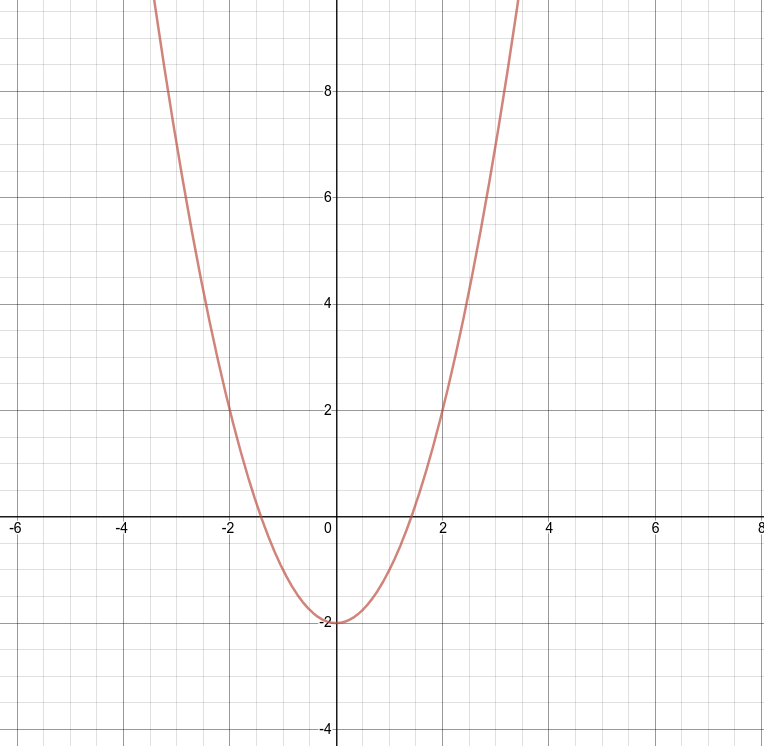
\includegraphics[scale=0.5]{Parabola.png}
    \caption{Grafico funzione $f(x)=x^2-2$}
\end{figure} \\
Come si può vedere dal grafico di questa funzione, abbiamo che le due radici sono negli intervalli $[-2,0]$ e $[0,2]$.
Questo risultato si può ottenere teoricamente andando ad applicare a questi estremi il teorema dell'esistenza degli zeri.
Dopo aver determinato in quali intervalli sono le due radici, possiamo andare ad utilizzare i metodi per la ricerca degli zeri di una funzione.
Nei vari metodi, andremo alla ricerca della radice nell'intervallo $[0;2]$ usando come tolleranza $10^{-8}$ e numero massimo di iterazioni pari a $100$.
\newpage
\subsubsection{Metodo di bisezione}
Con il metodo di bisezione, andando a dare come parametri $f(x)=x^2-2$ e $[a,b]=[0;2]$ otteniamo:
\begin{figure}[ht!]
    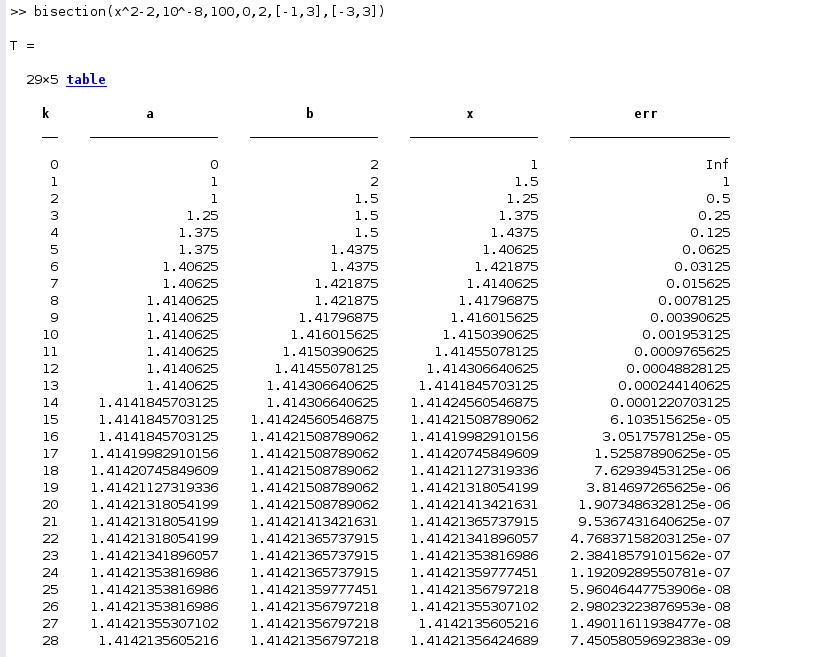
\includegraphics[scale=0.63]{TabellaParabolaBisezione.png}
    \caption{Tabella Metodo di Bisezione su $f(x)=x^2-2$}
\end{figure}
\begin{figure}[ht!]
    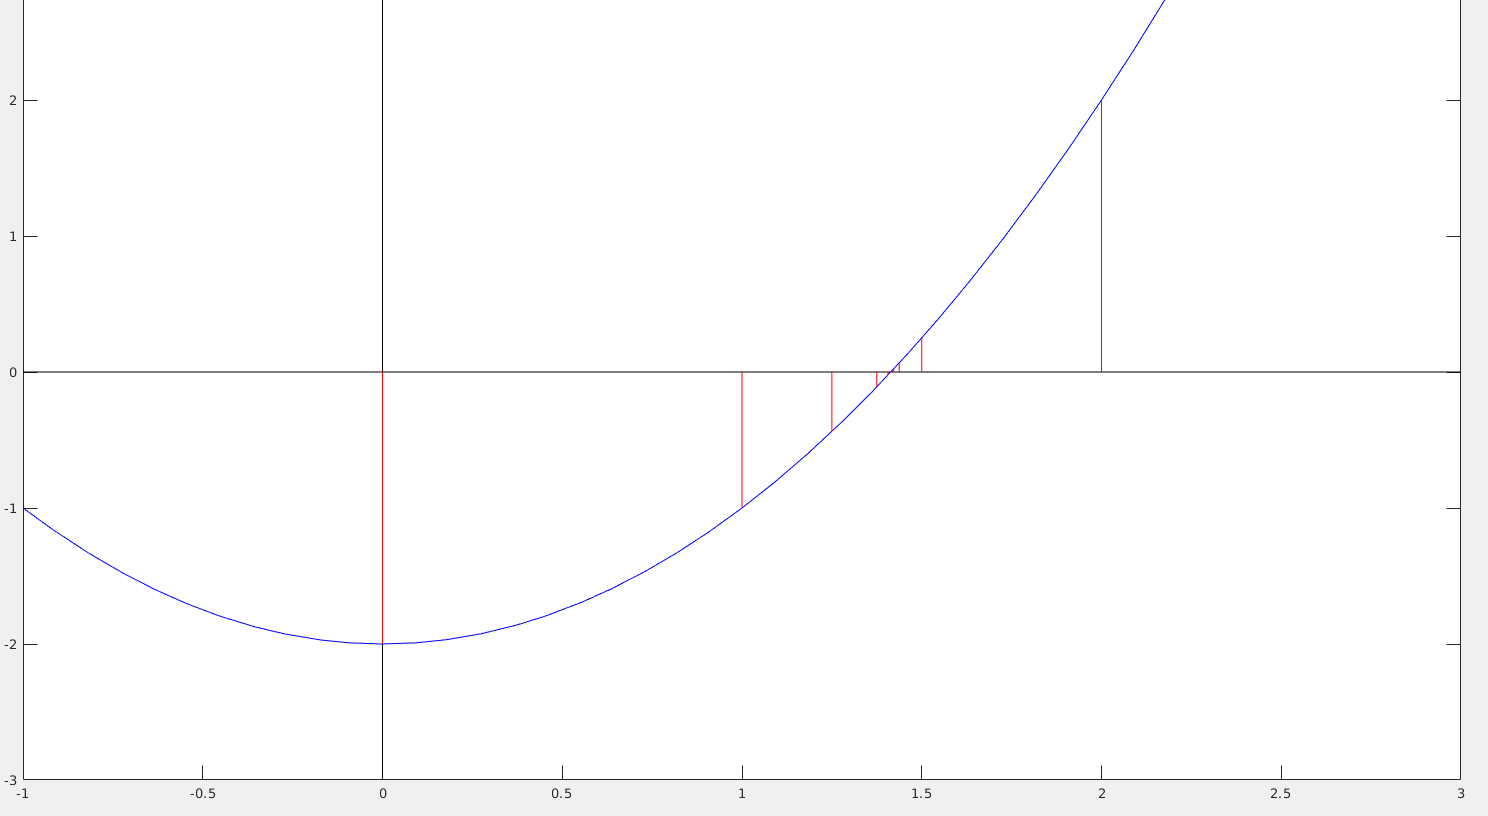
\includegraphics[scale=0.4]{ParabolaBisezione.png} 
    \caption{Grafico Metodo di Bisezione su $f(x)=x^2-2$}
\end{figure}

Questi sono i risultati ottenuti dall'esecuzione del programma in MATLAB.\\ Come si può vedere, l'algoritmo esegue 28 iterazioni andando a passare come parametro una tolleranza pari a $10^{-8}$.
Nelle varie iterazioni, il metodo di Bisezione si avvicina sempre di più alla radice, restrigendo l'intervallo e spostando gli estremi (Nel grafico segnati con la linea rossa). \\
Infine si ottiene che la radice della funzione \'e approssimativamente $\sqrt{2}$.

\subsubsection{Metodo di punto fisso}
Con il metodo di punto fisso, andando a dare come parametri $g(x)=\frac{2}{x}$ e $x_0=1.5$ otteniamo:
\begin{figure}[ht!]
    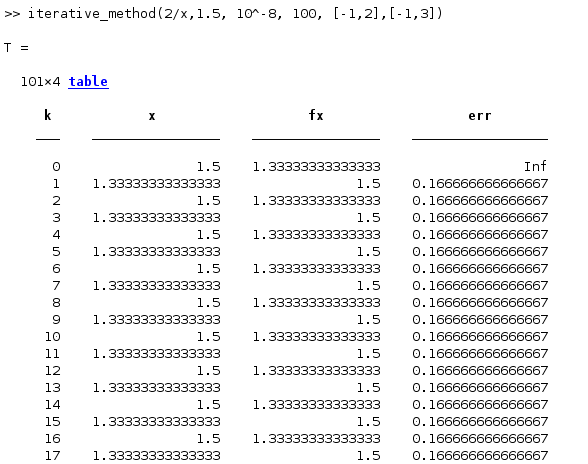
\includegraphics[scale=0.60]{TabellaParabolaPuntoFisso.png}
    \caption{Tabella Metodo di Punto Fisso su $g(x)=\frac{2}{x}$ }
\end{figure}
\begin{figure}[ht!]
    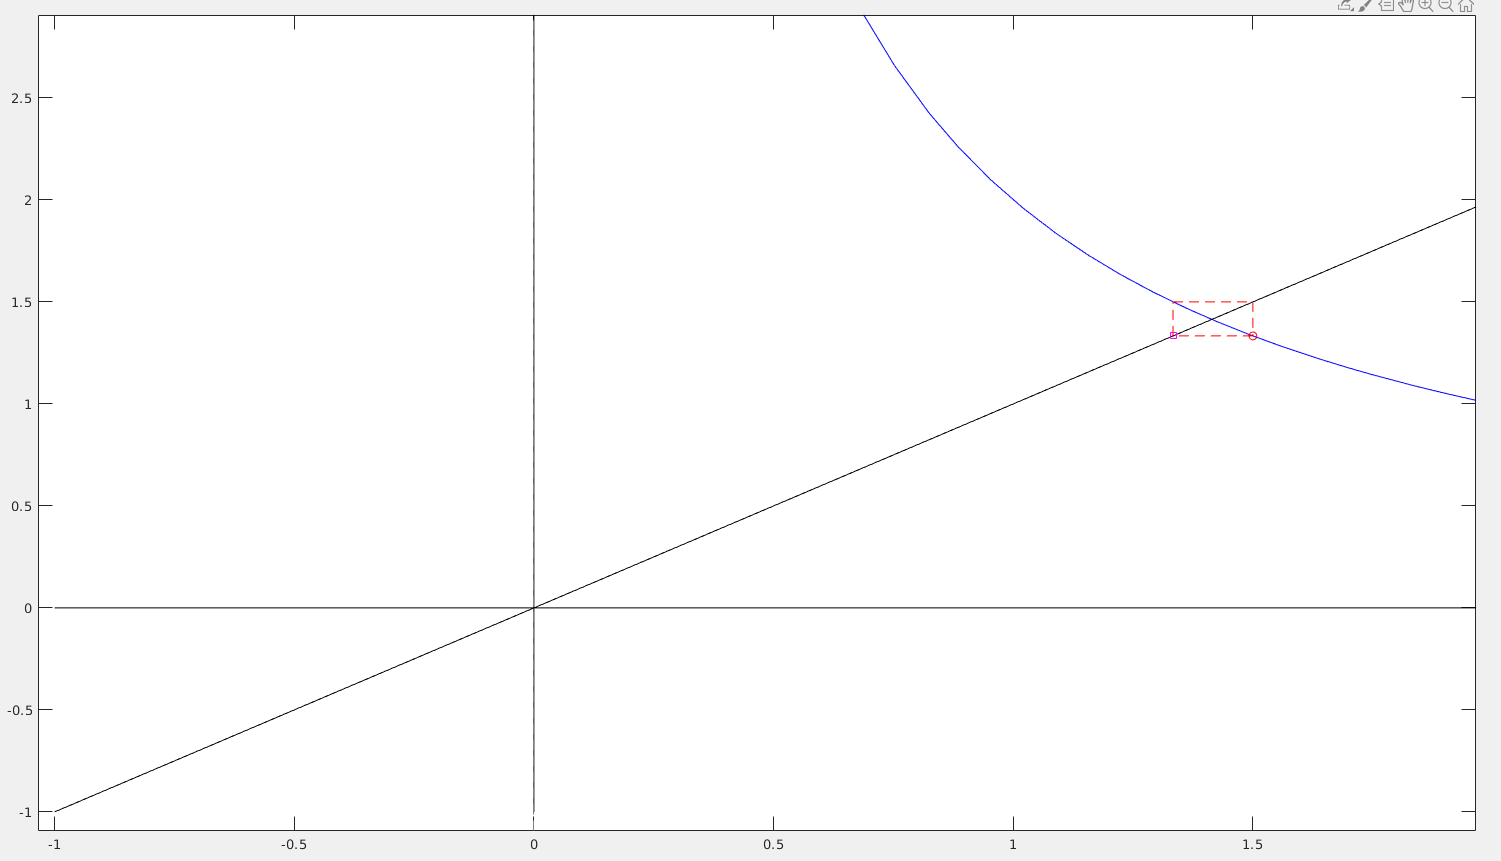
\includegraphics[scale=0.39]{ParabolaPuntoFisso.png} 
    \caption{Grafico Metodo di Punto Fisso su $g(x)=\frac{2}{x}$}
\end{figure} \\

Questi sono i risultati ottenuti dall'esecuzione del programma in MATLAB.\\ Come si può vedere,il programma esegue sempre le solite operazioni in loop, infatti esso fa più delle 100 iterazioni massime.
Questo \'e giustificato dal fatto che se andiamo a studiare teoricamente la funzione $g(x)$ otteniamo che la sua derivata \'e: $g'(x)=-\frac{2}{x^2}$. Per il teorema 2 precedentemente esposto nella descrizione del punto fisso, abbiamo che la successione
converge localmente se in un intorno di $\xi$ vale $-1<g'(x)<1$, ma non è questo il caso perchè la $g'(x)$ è monotona decrescente a sinistra di $\xi$ dove $g'(\sqrt{2})=1$, quindi non ho convergenza in $\xi$ perchè non ho intorni che soddisfano la definizione di convergenza locale. 
\newpage

\subsubsection{Metodo di Newton}
Con il metodo di Newton, andando a dare come parametri $f(x)=x^2-2$ e $x_0=2$ otteniamo:
\begin{figure}[ht!]
    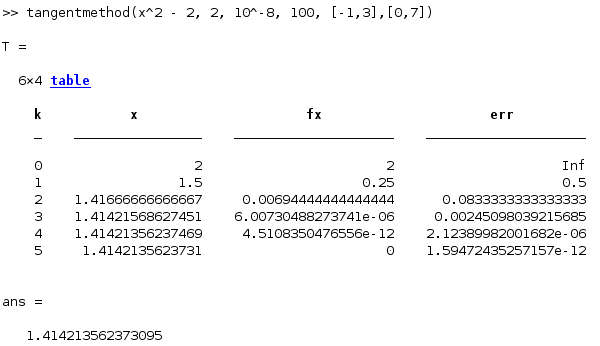
\includegraphics[scale=0.63]{TabellaParabolaNewton.png}
    \caption{Tabella Metodo di Newton su $f(x)=x^2-2$}
\end{figure}
\begin{figure}[ht!]
    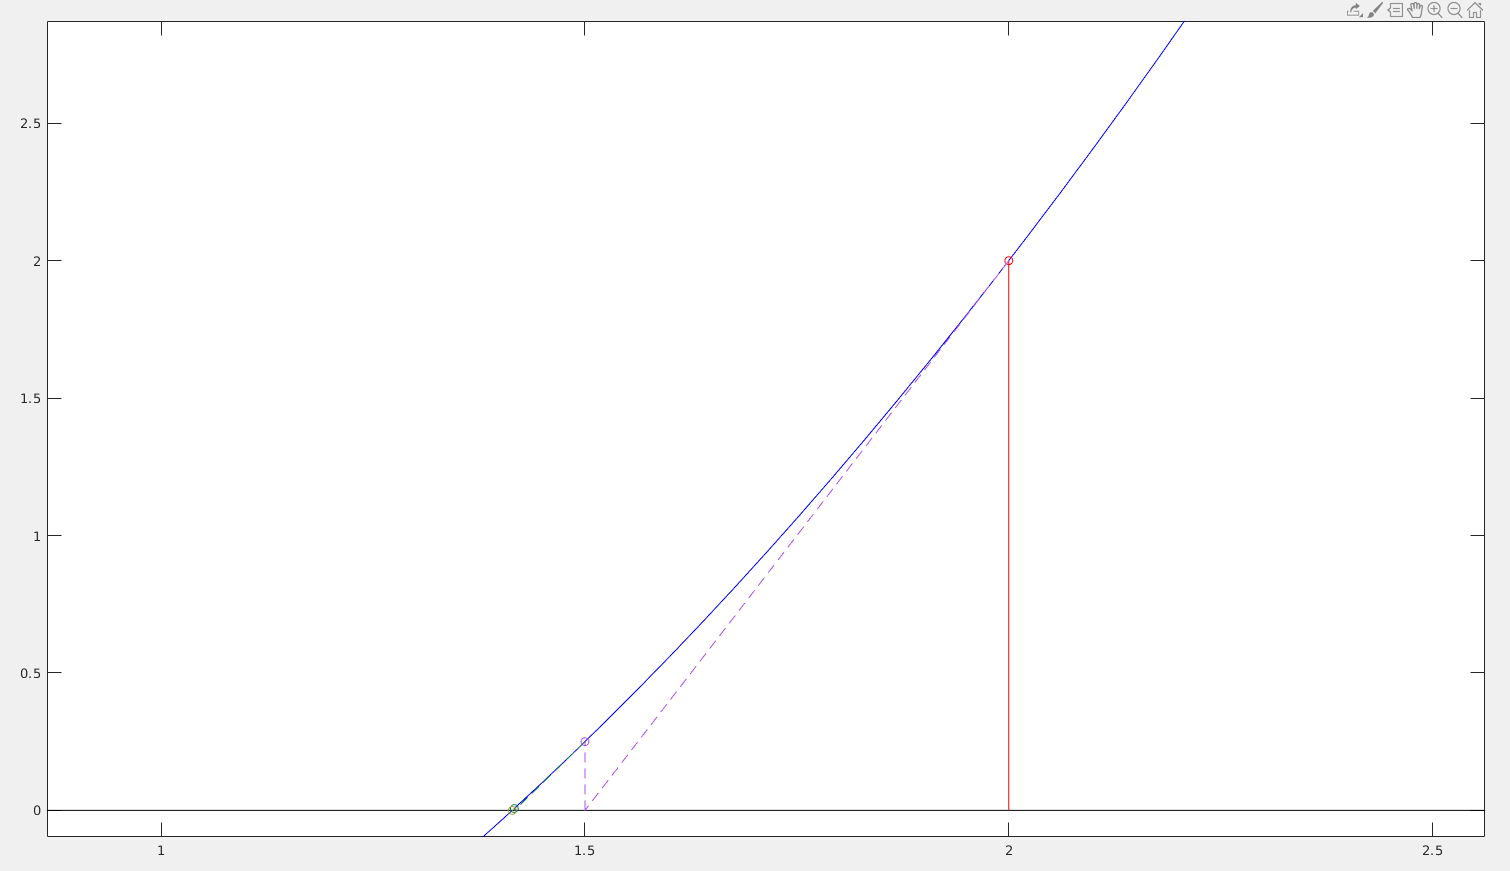
\includegraphics[scale=0.44]{ParabolaNewton.png}
    \caption{Grafico Metodo di Newton su $f(x)=x^2-2$}
\end{figure} \\
Questi sono i risultati ottenuti dall'esecuzione del programma in MATLAB.\\ Come si può vedere,l'algoritmo esegue 5 iterazioni andando a passare come parametro una tolleranza pari a $10^{-8}$.
Questo \'e giustificato teoricamente dato che per il teorema $4$, precedentemente esposto, che se $f(\xi)=0$, $\xi \in (a,b)$ e $f \in \mathtt{C}^2[(a,b)]$, se $f'(\xi) \neq 0 \implies$ Il metodo di Newton \'e localmente convergente ad $\xi$.
Infatti la derivata di $f(x)=x^2-2$ \'e $f'(x)=2x$, quindi $f'(\xi)=2*\sqrt{2}\neq 0$ quindi c'\'e convergenza locale in $\xi$.

\subsubsection{Metodo delle Corde}
Con il metodo delle Corde, andando a dare come parametri $f(x)=x^2-2$ e $x_0=2$ otteniamo:
\begin{figure}[ht!]
    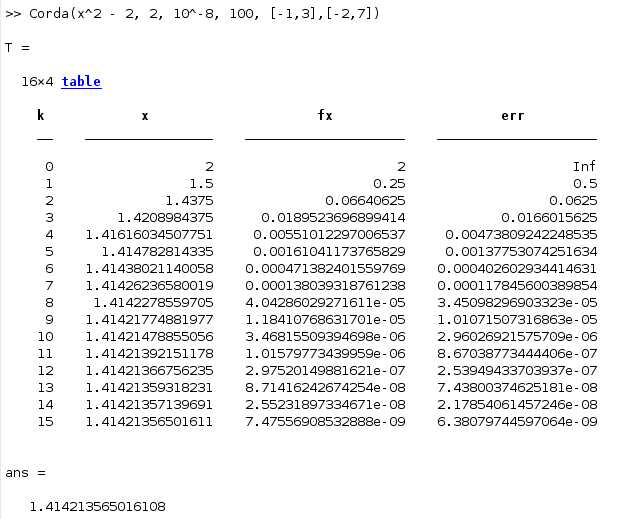
\includegraphics[scale=0.63]{TabellaParabolaCorda.png}
    \caption{Tabella Metodo della Corda su $f(x)=x^2-2$}
\end{figure}
\begin{figure}[ht!]
    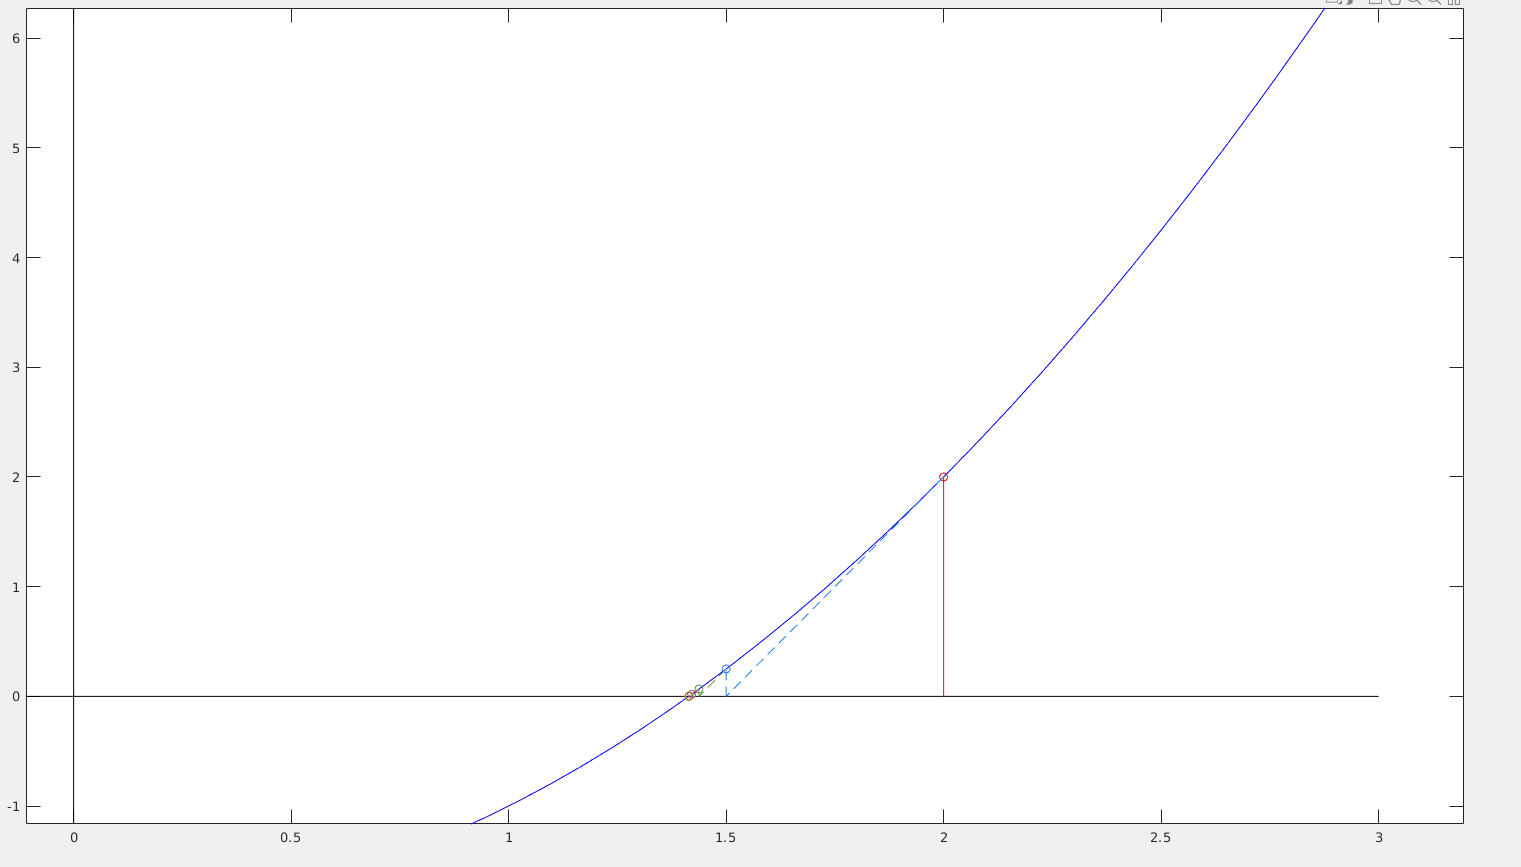
\includegraphics[scale=0.5]{ParabolaChord.png}
    \caption{Grafico Metodo della Corda su $f(x)=x^2-2$}
\end{figure} \\

Questi sono i risultati ottenuti dall'esecuzione del programma in MATLAB.\\ Come si può vedere, l'algoritmo esegue 15 iterazioni andando a passare come parametro una tolleranza pari a $10^{-8}$.
Il risultato \'e dovuto al fatto che non va ad aggiornare $f'(x)$ ogni volta, ma lo calcola solo inizialmente. Quindi avendo la sempre la solita derivata, ci mette più iterazioni rispetto al metodo di Newton.

\subsubsection{Metodo delle Secanti}
Con il metodo delle Secanti, andando a dare come parametri $f(x)=x^2-2$, $x_0=2$ e $x_1$=3 otteniamo:
\begin{figure}[ht!]
    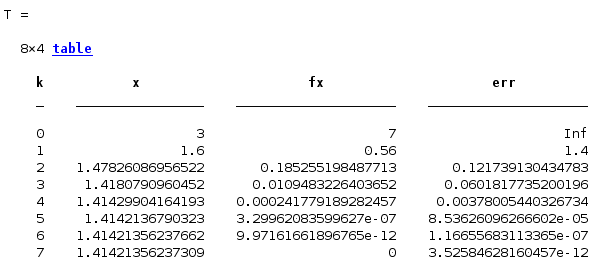
\includegraphics[scale=0.6]{TabellaParabolaSecant.png}
    \caption{Tabella Metodo delle Secanti su $f(x)=x^2-2$}
\end{figure}
\begin{figure}[ht!]
    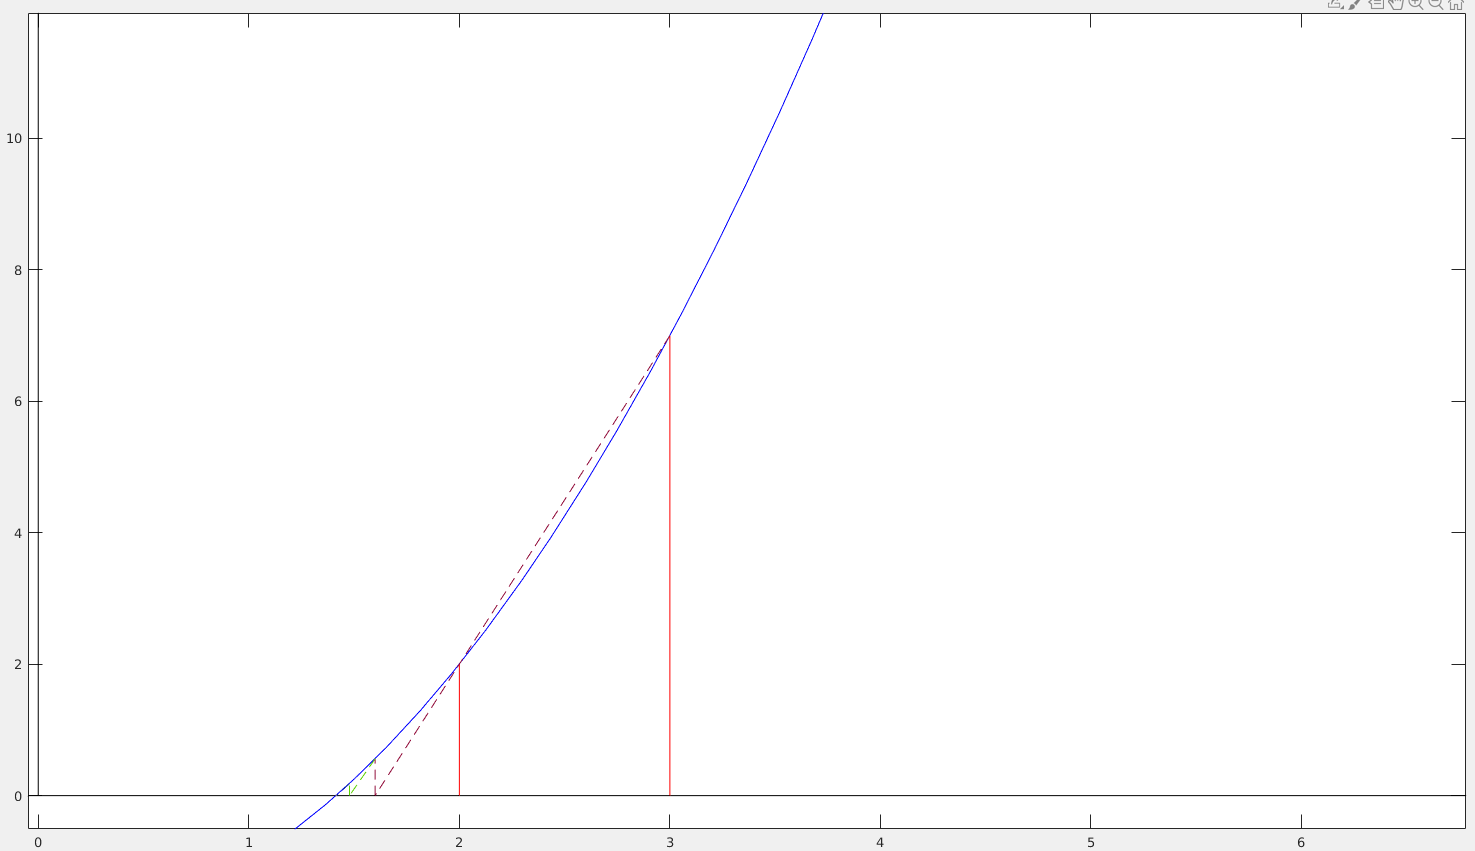
\includegraphics[scale=0.42]{ParabolaSecant.png}
    \caption{Grafico Metodo delle Secanti  su $f(x)=x^2-2$}
\end{figure} \\

Questi sono i risultati ottenuti dall'esecuzione del programma in MATLAB.\\ Come si può vedere,l'algoritmo esegue 7 iterazioni andando a passare come parametro una tolleranza pari a $10^{-8}$.
Usando due punti iniziali, riesce ad approssimare, come si \'e visto precedentemente nell'introduzione dei vari metodi, con velocit\'a di convergenza superlineare, quindi più veloce rispetto al metodo delle corde.

\newpage

\subsection{Secondo caso di applicazione: $f(x)=e^{-x}-2x^2$}
Come secondo caso di applicazione utilizziamo una funzione più complessa rispetto alla precedente.
\begin{figure}[ht!]
    \centering
    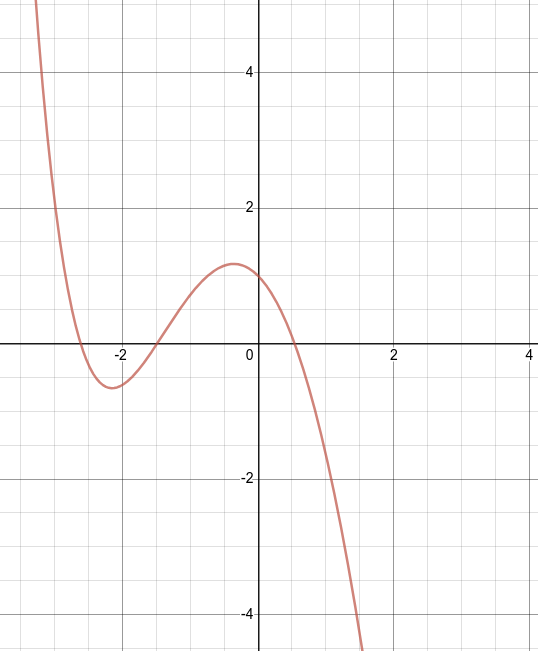
\includegraphics[scale=0.6]{Esponenziale.png}
    \caption{Grafico funzione $f(x)=e^{-x}-2x^2$}
\end{figure} \\

Come si può vedere dal grafico di questa funzione, abbiamo $3$ radici negli intervalli $[-3,-2]$,$[-2,-1]$,$[0,1]$.
Questo risultato si può ottenere teoricamente andando ad applicare a questi estremi il teorema dell’esistenza degli zeri.
Dopo aver determinato in quali intervalli sono le tre radici, possiamo andare ad utilizzare i metodi per la ricerca degli zeri di una funzione.
Andremo a studiare come testing la radice nell'intervallo $[-2,-1]$ usando come tolleranza $10^{-8}$ e numero massimo di iterazioni pari a $100$.
\newpage
\subsubsection{Metodo di bisezione}
Con il metodo di bisezione, andando a dare come parametri $f(x)=e^{-x}-2x^2$ e $[a,b]=[-2,0]$ otteniamo:
\begin{figure}[ht!]
    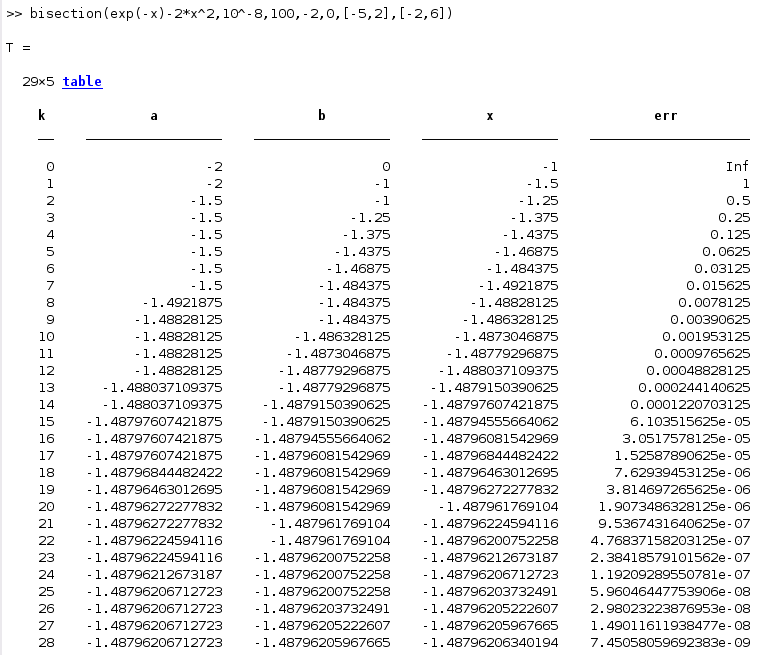
\includegraphics[scale=0.63]{TabellaEsponenzialeBisezione.png}
    \caption{Tabella Metodo di bisezione su $f(x)=e^{-x}-2x^2$}
\end{figure}
\begin{figure}[ht!]
    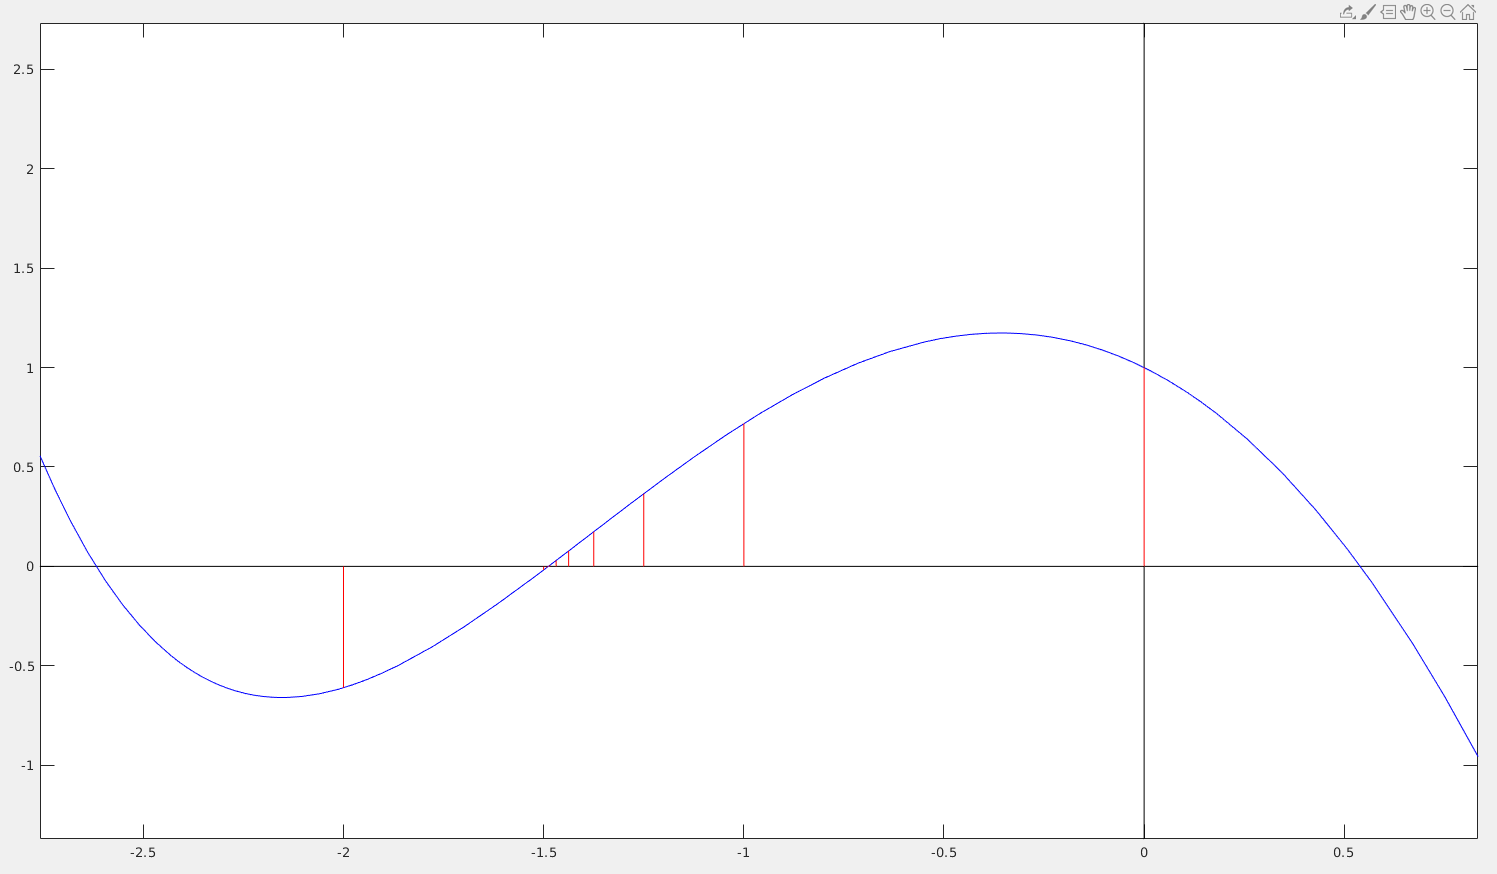
\includegraphics[scale=0.4]{EsponenzialeBisezione.png}
    \caption{Grafico Metodo di bisezione su $f(x)=e^{-x}-2x^2$}
\end{figure} \\

Questi sono i risultati ottenuti dall'esecuzione del programma in MATLAB.\\ Come si può vedere, l'algoritmo esegue 28 iterazioni andando a passare come parametro una tolleranza pari a $10^{-8}$.
Nelle varie iterazioni, il metodo di Bisezione si avvicina sempre di più alla radice, restrigendo l'intervallo e spostando gli estremi (Nel grafico riportati con la linea rossa). \\
Infine si ottiene che la radice della funzione \'e approssimativamente $-1.487$.

\newpage

\subsubsection{Metodo di punto fisso}
Con il metodo di punto fisso, andando a dare come parametri $g(x)=\frac{e^{-x}}{2x}$ e $x_0=-0.3$ otteniamo:
\begin{figure}[ht!]
    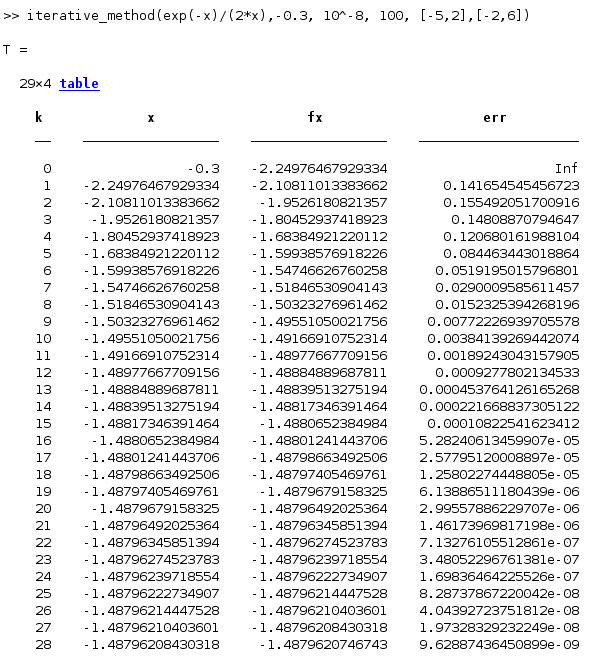
\includegraphics[scale=0.63]{TabellaEsponenzialePuntoFisso.png}
    \caption{Tabella Metodo di Punto Fisso su $g(x)=\frac{e^{-x}}{2x}$}
\end{figure}
\begin{figure}[ht!]
    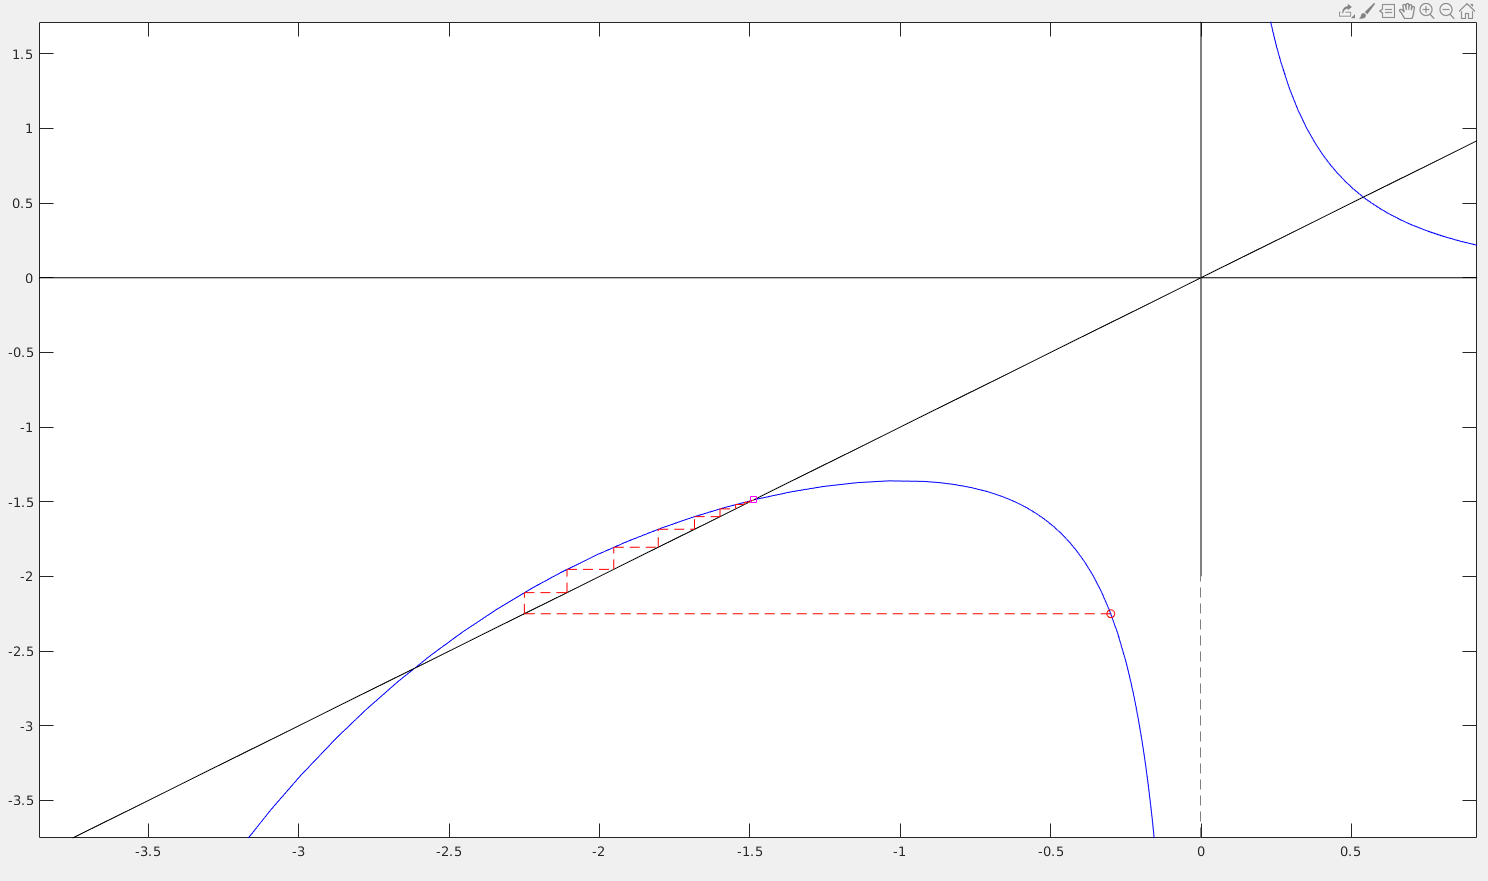
\includegraphics[scale=0.4]{EsponenzialePuntoFisso.png}
    \caption{Grafico Metodo di Punto Fisso su $g(x)=\frac{e^{-x}}{2x}$}
\end{figure} \\


Questi sono i risultati ottenuti dall'esecuzione del programma in MATLAB.\\ Come si può vedere, l'algoritmo esegue 28 iterazioni andando a passare come parametro una tolleranza pari a $10^{-8}$.
Questo \'e giustificato dal fatto che se andiamo a studiare teoricamente la funzione $g(x)$ otteniamo che la sua derivata \'e: $g'(x)=-\frac{2}{x^2}$. 
Studiando il grafico della derivata, scopriremo che \'e monotona decrescente nell'intervallo $[-2,-1]$, andando a valutare la derivata negli estremi dell'intervallo, otterremo che $f'(-2)=0.924$ e $f'(-1)=0$.
Per il teorema del Punto Fisso esposto nella descrizione del omonimo metodo, otteniamo quindi la convergenza locale perch\'e $-1<g'(x)<1$ in tutti i punti compresi nell'intervallo $[-2,-1]$.


\subsubsection{Metodo di Newton}
Con il metodo di Newton, andando a dare come parametri $f(x)=e^{-x}-2x^2$ e $x_0=-1$ otteniamo:
\begin{figure}[ht!]
    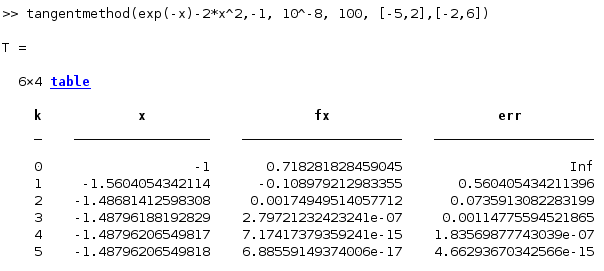
\includegraphics[scale=0.63]{TabellaEsponenzialeNewton.png}
    \caption{Tabella Metodo di Newton su $f(x)=e^{-x}-2x^2$}
\end{figure}
\begin{figure}[ht!]
    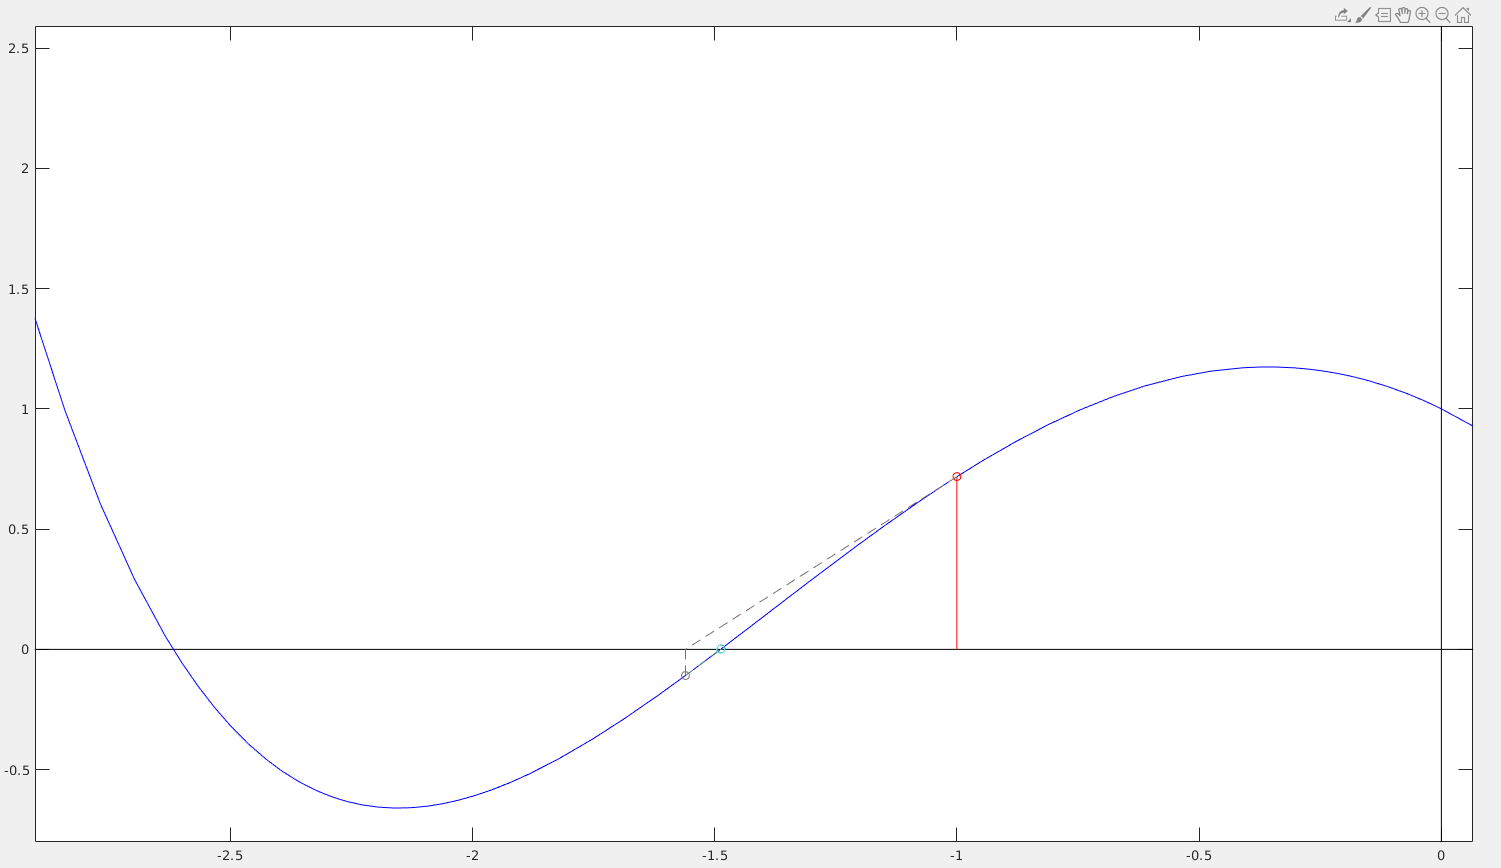
\includegraphics[scale=0.4]{EsponenzialeNewton.png}
    \caption{Grafico Metodo di Newton su $f(x)=e^{-x}-2x^2$}
\end{figure} \\


Questi sono i risultati ottenuti dall'esecuzione del programma in MATLAB.\\ Come si può vedere,l'algoritmo esegue 5 iterazioni andando a passare come parametro una tolleranza pari a $10^{-8}$.
Questo \'e giustificato teoricamente perch\'e sappiamo che, per il teorema $4$, se $f(\xi)=0$, $\xi \in (a,b)$ e $f \in \mathtt{C}^2[(a,b)]$, se $f'(\xi) \neq 0 \implies$ Il metodo di Newton \'e localmente convergente a $\xi$.
Infatti la derivata di $f(x)=e^{-x}-2x^2$ \'e $f'(x)=-e^{-x}-4x$, andando a studiare il grafico della derivata, scopriremo che $f'(x)>0, \; \forall \, x \in [-2,-1]$ quindi anche $f'(\xi) \neq 0$. 

\subsubsection{Metodo delle Corde}
Con il metodo delle Corde, andando a dare come parametri $f(x)=e^{-x}-2x^2$ e $x_0=-1$ otteniamo: 
\begin{figure}[ht!]
    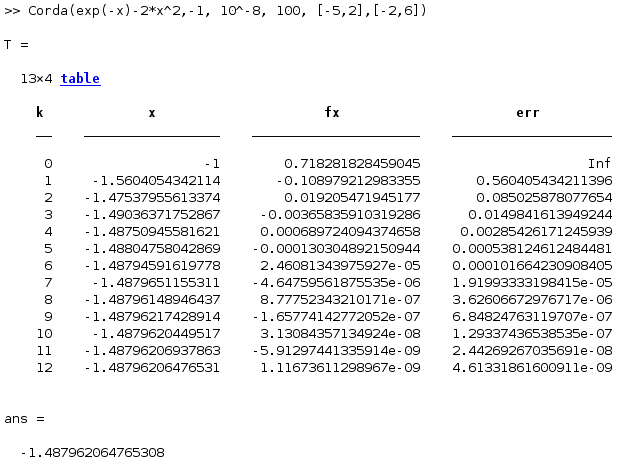
\includegraphics[scale=0.59]{TabellaEsponenzialeChord.png}
    \caption{Tabella Metodo delle Corde su $f(x)=e^{-x}-2x^2$}
\end{figure}
\begin{figure}[ht!]
    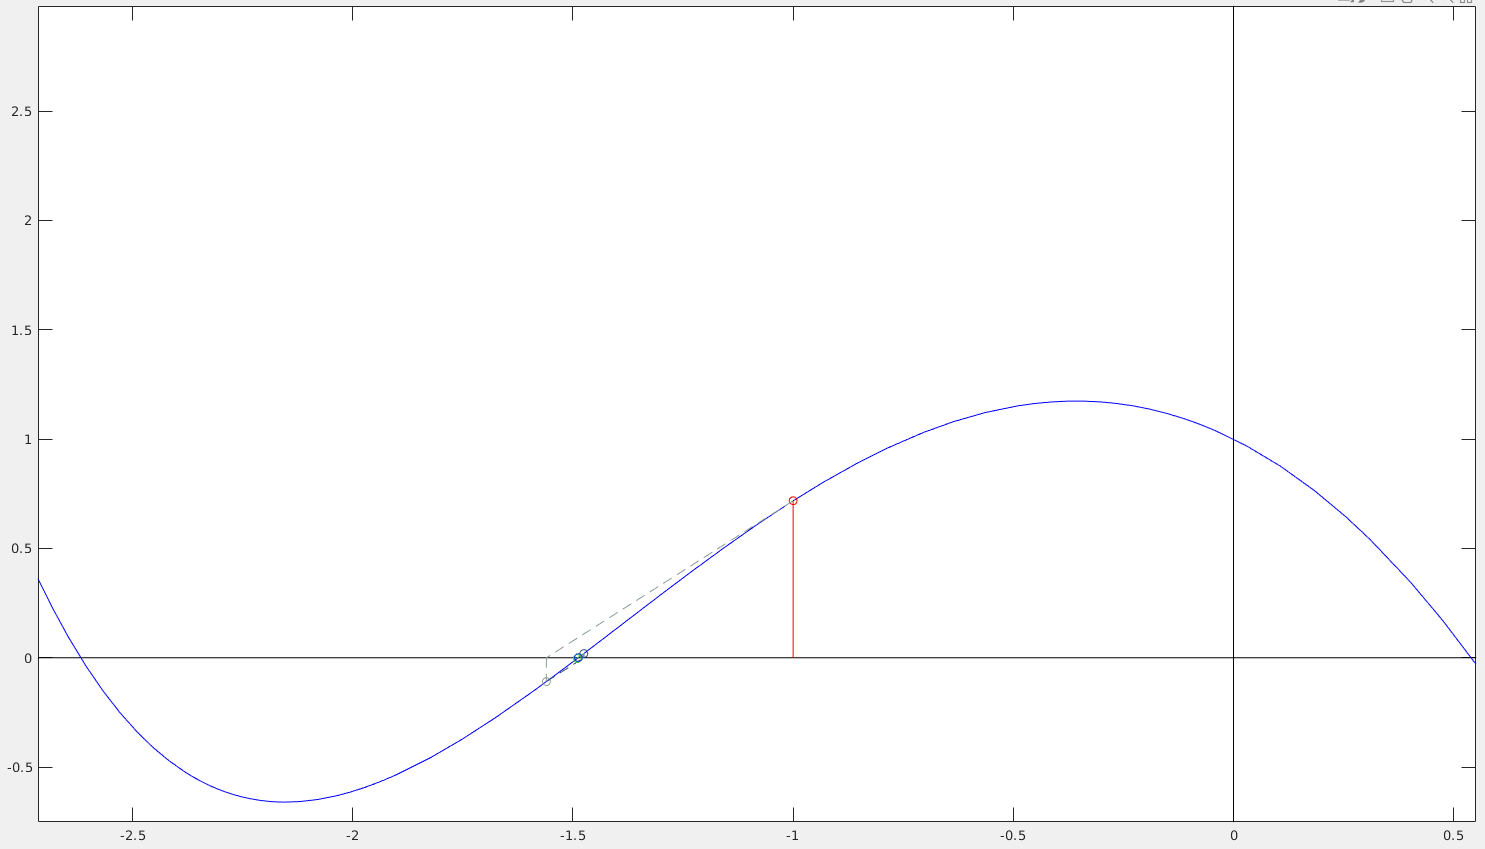
\includegraphics[scale=0.40]{EsponenzialeChord.png}
    \caption{Grafico Metodo delle Corde su $f(x)=e^{-x}-2x^2$}
\end{figure} \\



Questi sono i risultati ottenuti dall'esecuzione del programma in MATLAB.\\ Come si può vedere,l'algoritmo esegue 12 iterazioni andando a passare come parametro una tolleranza pari a $10^{-8}$.
Il risultato \'e dovuto al fatto che non va ad aggiornare $f'(x)$ ad ogni iterazione, ma lo calcola solo inizialmente. Quindi avendo la medesima derivata, ci impiega più iterazioni rispetto al metodo di Newton.    

\subsubsection{Metodo delle Secanti}
Con il metodo delle Secanti, andando a dare come parametri $f(x)=e^{-x}-2x^2$ e $x_0=-1$, $x_1=-0.9$ otteniamo:
\begin{figure}[ht!]
    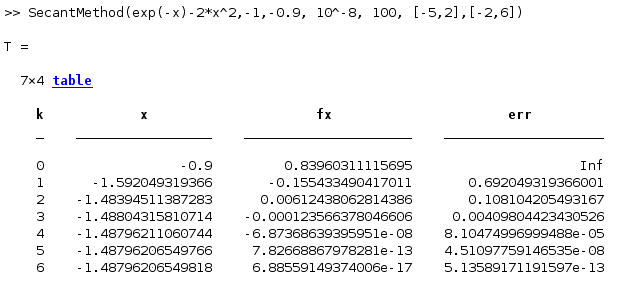
\includegraphics[scale=0.60]{TabellaEsponenzialeSecant.png}
    \caption{Tabella Metodo delle Secanti su $f(x)=e^{-x}-2x^2$}
\end{figure}
\begin{figure}[ht!]
    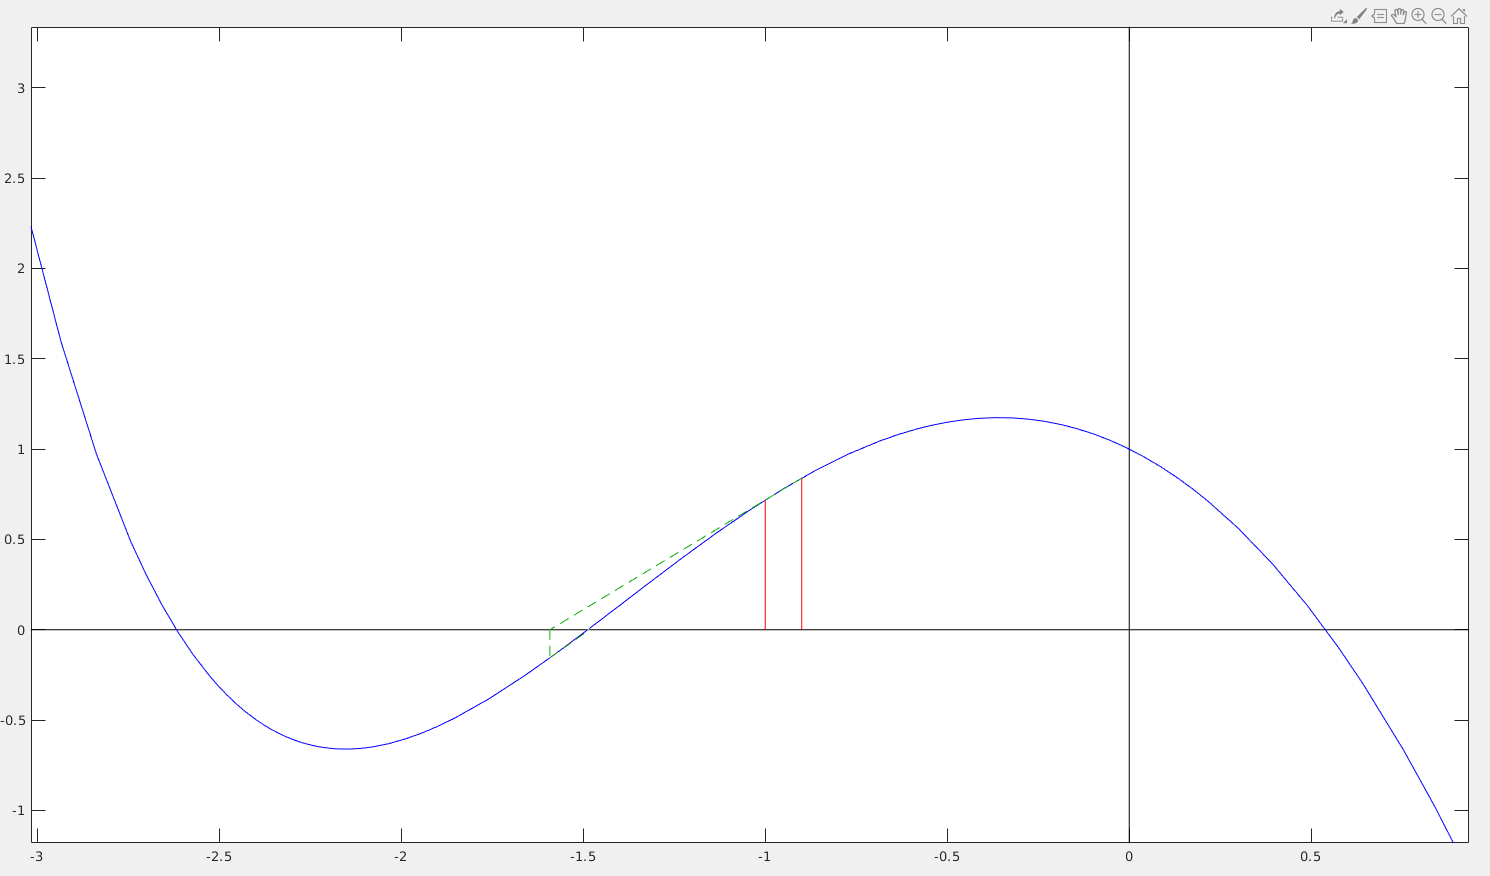
\includegraphics[scale=0.40]{EsponenzialeSecant.png}
    \caption{Grafico Metodo delle Secanti su $f(x)=e^{-x}-2x^2$}
\end{figure} \\

Questi sono i risultati ottenuti dall'esecuzione del programma in MATLAB.\\ Come si può vedere,l'algoritmo esegue 6 iterazioni andando a passare come parametro una tolleranza pari a $10^{-8}$.
Usando due punti iniziali, riesce ad approssimare, come prima riportato, con velocit\'a di convergenza superlineare, quindi più veloce rispetto al metodo delle corde.

\newpage

\subsection{Terzo caso di applicazione: $f(x)=x^5-3x^4+7x^3-13x^2+12x-4$}
Come terzo caso di applicazione utilizziamo una funzione la quale ha una radice tripla in 1.
\begin{figure}[ht!]
    \centering
    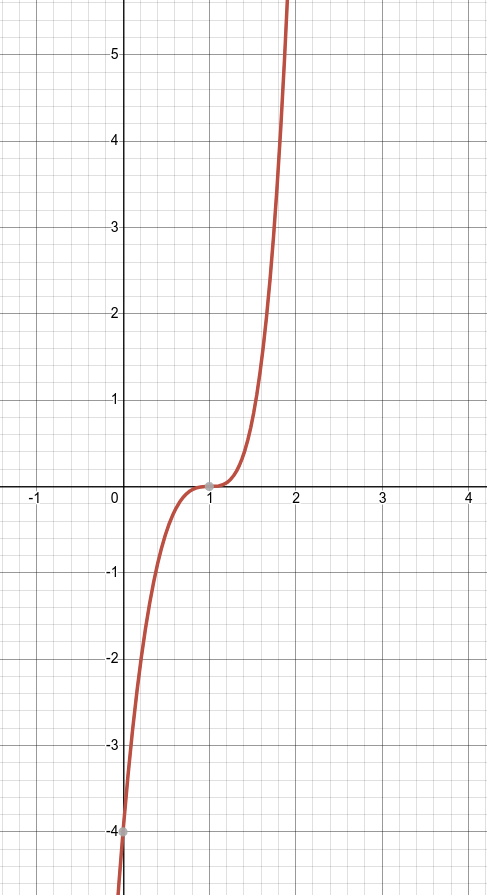
\includegraphics[scale=0.5]{MultiRadix.png}
    \caption{Grafico funzione $f(x)=x^5-3x^4+7x^3-13x^2+12x-4$}
\end{figure} \\
Andremo a studiare come testing la radice tripla in 1 usando come tolleranza $10^{-8}$ e numero massimo di iterazioni pari a $100$.
\newpage
\subsubsection{Metodo di bisezione}
Con il metodo di bisezione, andando a dare come parametri $f(x)=x^5-3x^4+7x^3-13x^2+12x-4$ e $[a,b]=[-2.5,2.5]$ otteniamo:
\begin{figure}[ht!]
    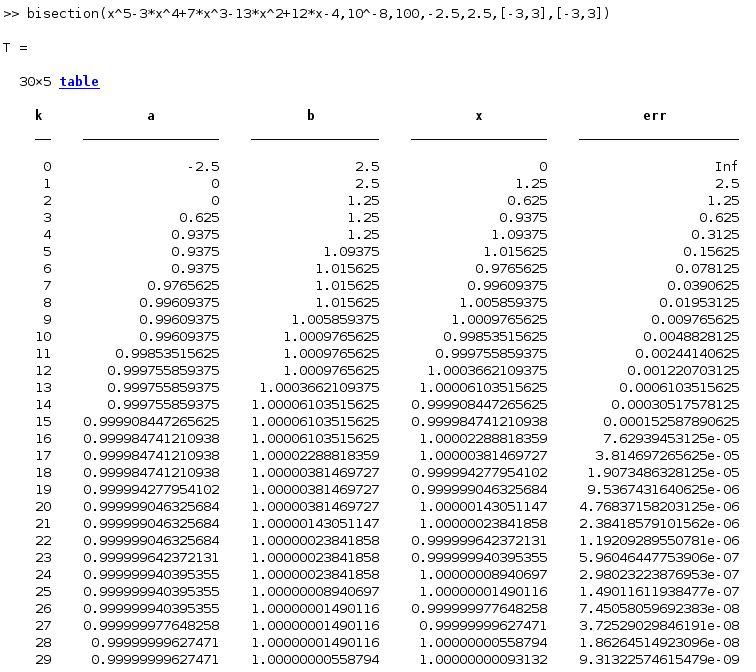
\includegraphics[scale=0.58]{TabellaMultiRadixBisezione.png}
    \caption{Tabella Metodo di bisezione su $f(x)=x^5-3x^4+7x^3-13x^2+12x-4$}
\end{figure}
\begin{figure}[ht!]
    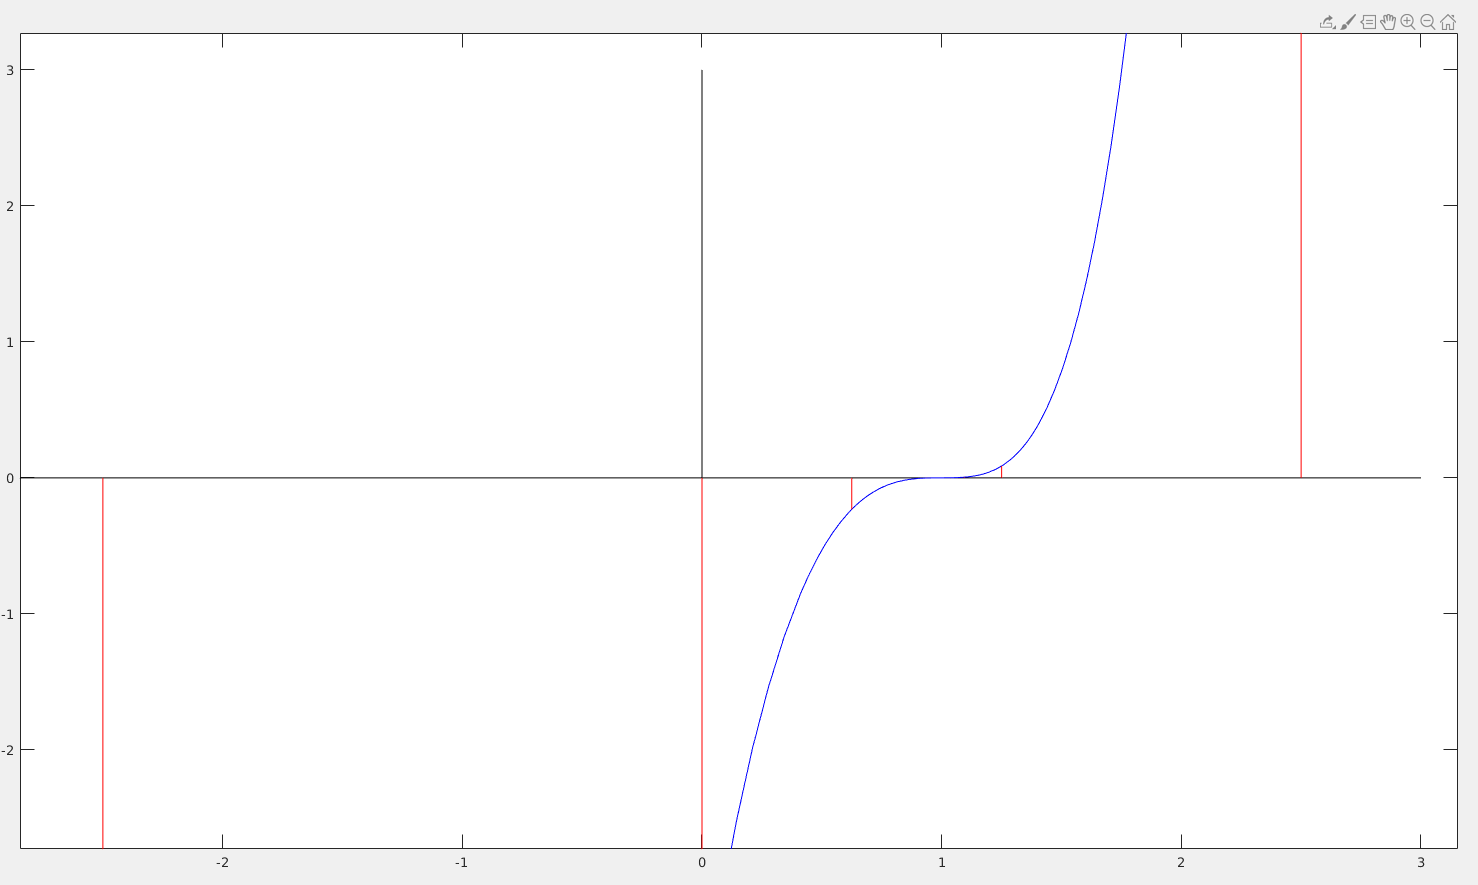
\includegraphics[scale=0.4]{MultiRadixBisezione1.png}
    \caption{Grafico Metodo di bisezione su $f(x)=x^5-3x^4+7x^3-13x^2+12x-4$}
\end{figure} \\
Questi sono i risultati ottenuti dall'esecuzione del programma in MATLAB.\\ Come si può vedere, l'algoritmo esegue 29 iterazioni andando a passare come parametro una tolleranza pari a $10^{-8}$.
Nelle varie iterazioni, il metodo di Bisezione si avvicina sempre di più alla radice, restrigendo l'intervallo e spostando gli estremi (Nel grafico evidenziati con la linea rossa). \\
Infine si ottiene che la radice della funzione \'e approssimativamente $1$.

\newpage

\subsubsection{Metodo di punto fisso}
Con il metodo di punto fisso, andando a dare come parametri $g(x)=\frac{3x^4-7x^3+13x^2-12x+4}{x^4}$ e $x_0=-1.5$ otteniamo:
\begin{figure}[ht!]
    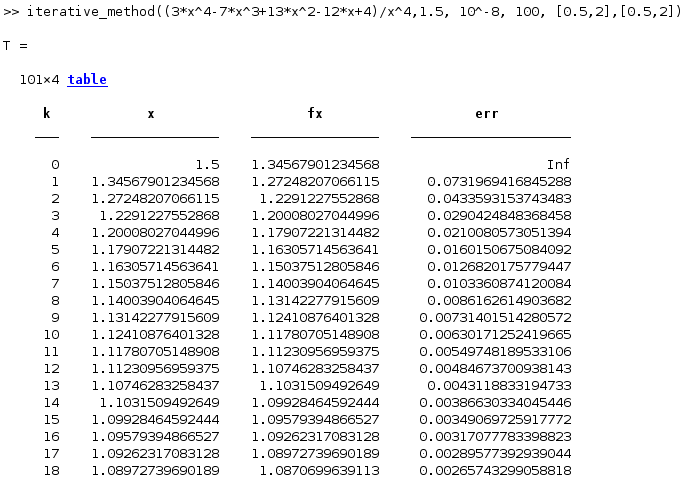
\includegraphics[scale=0.51]{TabellaMultiRadixPuntoFisso1.png}\\
    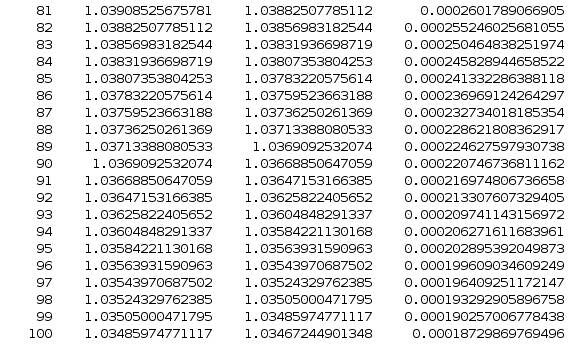
\includegraphics[scale=0.51]{TabellaMultiRadixPuntoFisso2.png}
    \caption{Tabella Metodo di Punto Fisso, iterazioni: 0-10, 81-100, su $g(x)=\frac{3x^4-7x^3+13x^2-12x+4}{x^4}$}
\end{figure}
\begin{figure}[ht!]
    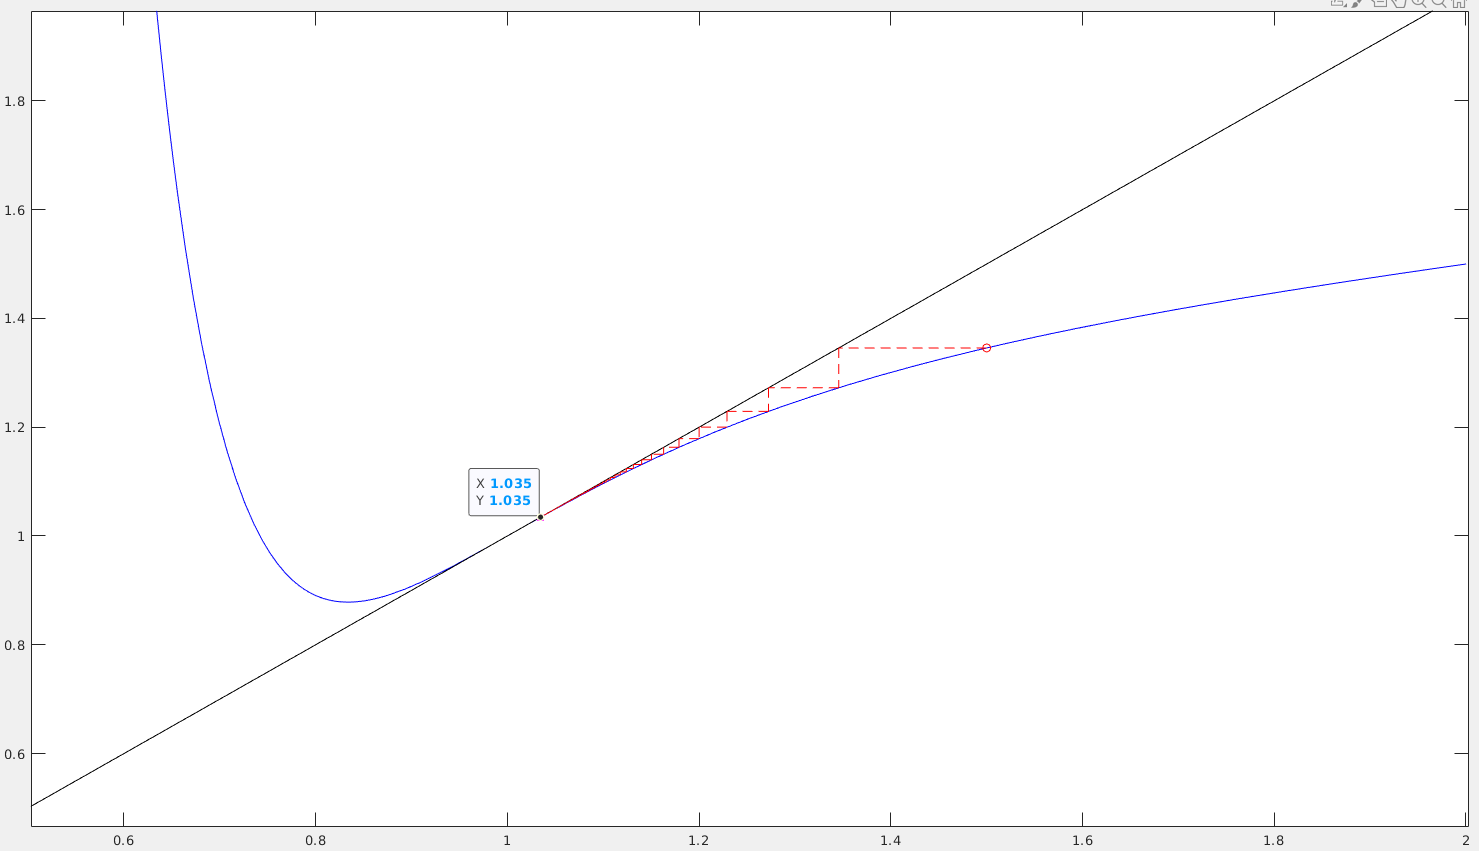
\includegraphics[scale=0.38]{MultiRadixPuntoFisso.png}
    \caption{Grafico Metodo di Punto Fisso su $g(x)=\frac{3x^4-7x^3+13x^2-12x+4}{x^4}$}
\end{figure}

\newpage

Questi sono i risultati ottenuti dall'esecuzione del programma in MATLAB.\\ Come si può vedere, l'algoritmo esegue più di 100 iterazioni andando a passare come parametro una tolleranza pari a $10^{-8}$.
Studiando teoricamente la convergenza locale ottengo che $g'(x)=\frac{7x^3-26x^2+36x-16}{x^5}$ la funzione ha un intorno di $\xi$ dove $-1<g'(x)<1$ però essendo che $g'(\xi)=1$ non posso dire nulla sulla sua convergenza per il teorema 3.


\subsubsection{Metodo di Newton}
Con il metodo di Newton, andando a dare come parametri $f(x)=x^5-3x^4+7x^3-13x^2+12x-4$ e $x_0=1.5$ otteniamo:
\begin{figure}[ht!]
    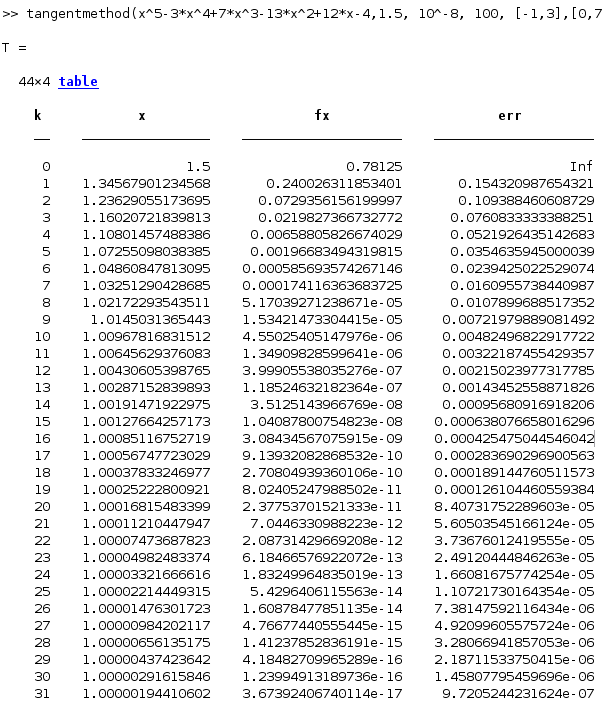
\includegraphics[scale=0.70]{TabellaMultiRadixNewton1.png}
    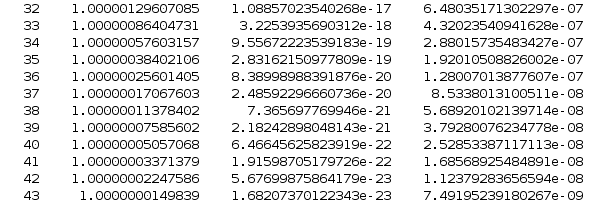
\includegraphics[scale=0.70]{TabellaMultiRadixNewton2.png}
    \caption{Tabella Metodo di Newton su $f(x)=x^5-3x^4+7x^3-13x^2+12x-4$}
\end{figure} \\
\begin{figure}[ht!]
    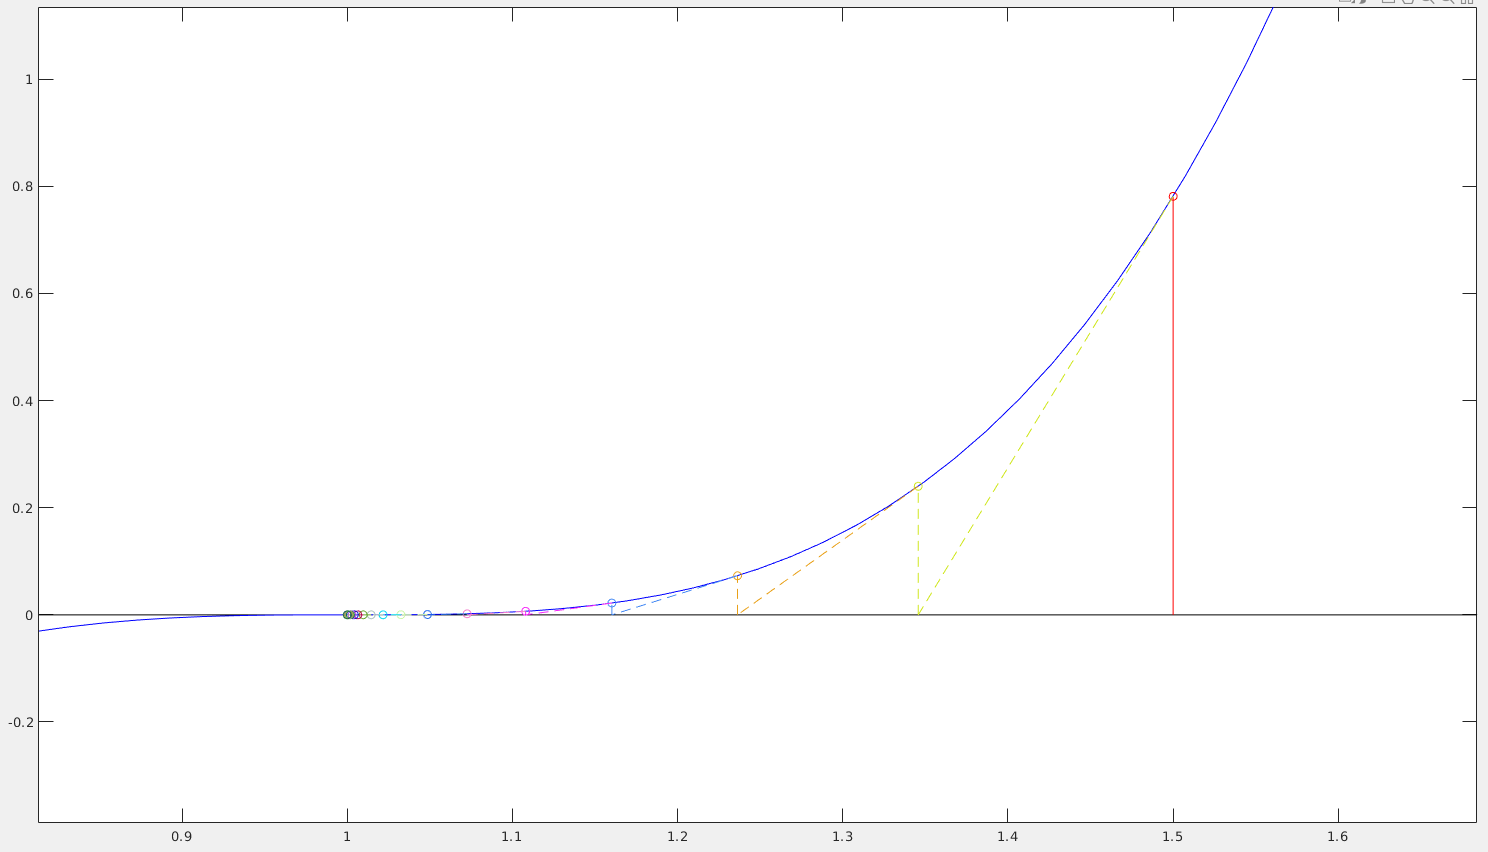
\includegraphics[scale=0.40]{MultiRadixNewton.png}
    \caption{Grafico Metodo di Newton su $f(x)=x^5-3x^4+7x^3-13x^2+12x-4$}
\end{figure}

Questi sono i risultati ottenuti dall'esecuzione del programma in MATLAB.\\ Come si può vedere,l'algoritmo esegue 43 iterazioni andando a passare come parametro una tolleranza pari a $10^{-8}$.
Questo \'e giustificato teoricamente perch\'e sappiamo che secondo il teorema $5$, sia $f:[a,b] \to \mathbb{R}$, $f(\xi)=0$, $\xi \in (a,b)$ e $f \in \mathtt{C}^2[(a,b)]$, se $\exists \delta>0: \forall \, x \in (\xi,\xi+\delta)=S \subset [a,b]$ si ha che:
se  $f'(x) \neq 0 $ e $f(x)*f''(x)>0 \, \forall \, x \in S \implies$ Il metodo di Newton \'e convergente a $\xi$ scegliendo $x_0 \in S$.
Andando a studiare la funzione per un intervallo $(\xi,\xi+\delta)=S$ o $(\xi-\delta,\xi)=S$ con $\delta \neq 0$ sappiamo che $\forall x \in S $, $ f'(x) \neq 0$ e $f(x)*f''(x)>0$, quindi c'è convergenza. Di seguito il grafico che mostra le varie funzioni:
\begin{figure}[ht!]
    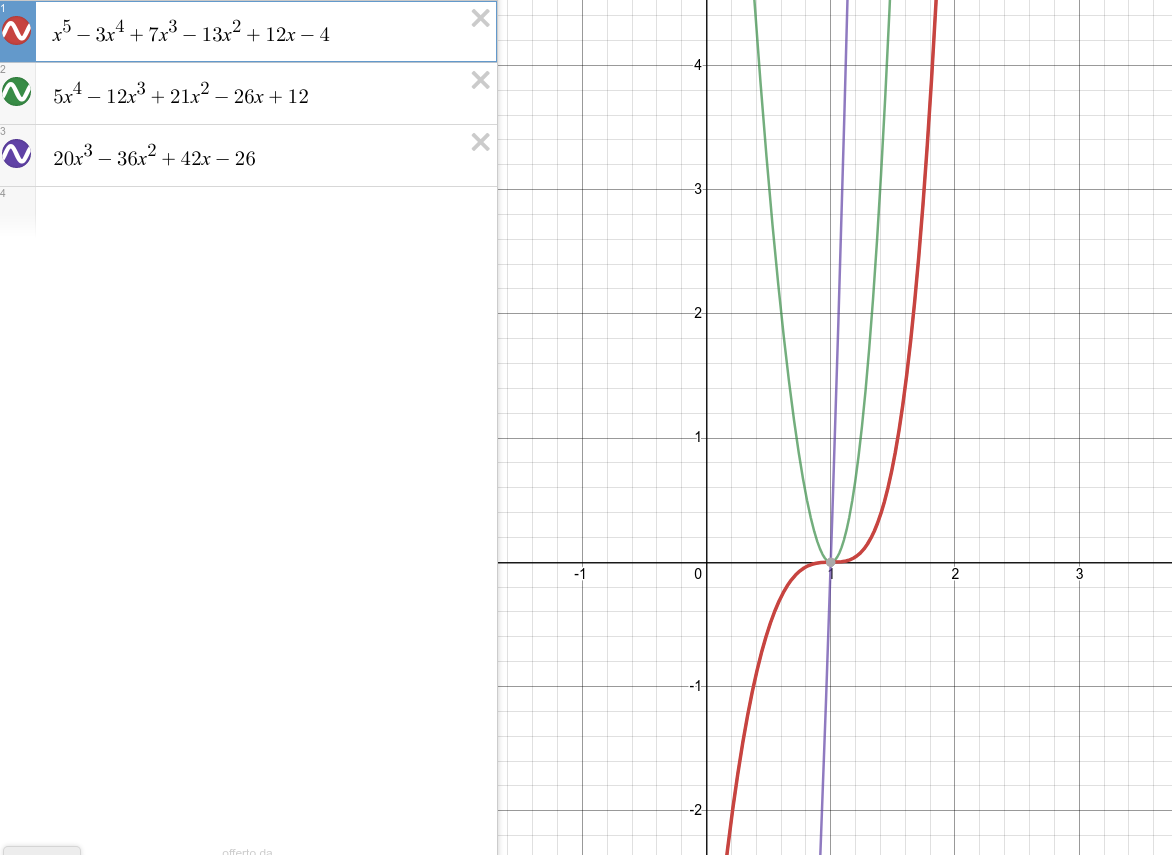
\includegraphics[scale=0.38]{MultiRadixGraficoNewton.png}
    \caption{Grafico delle funzione $f(x),f'(x),f''(x)$}
\end{figure}

\newpage

\subsubsection{Metodo delle Corde}
Con il metodo delle Corde, andando a dare come parametri $f(x)=x^5-3x^4+7x^3-13x^2+12x-4$ e $x_0=1.5$ otteniamo: 
\begin{figure}[ht!]
    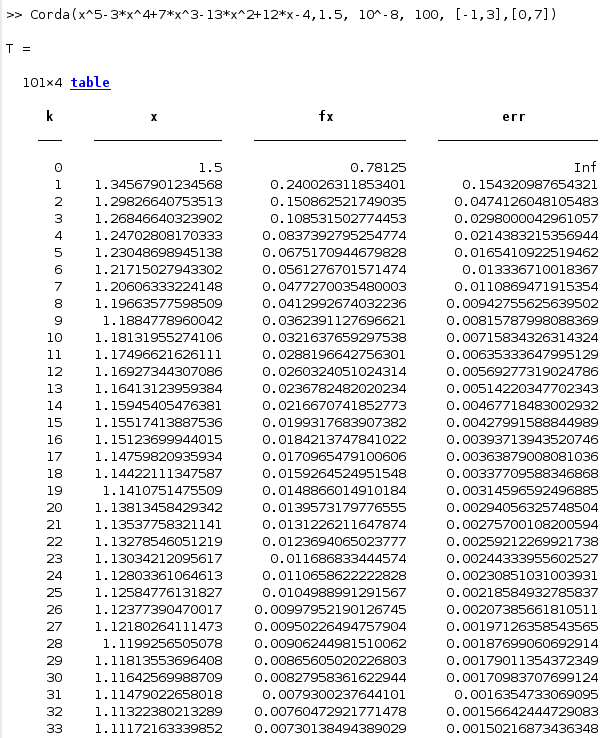
\includegraphics[scale=0.74]{TabellaMultiRadixCorda1.png} \\
    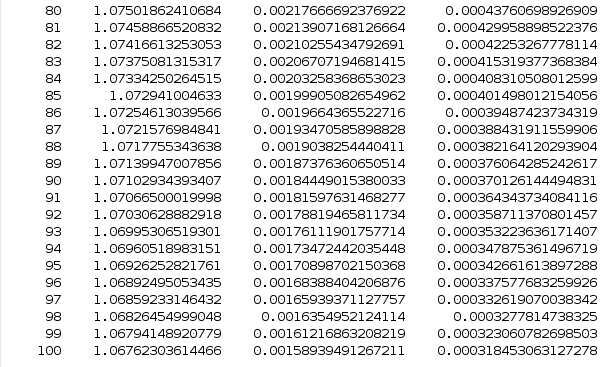
\includegraphics[scale=0.74]{TabellaMultiRadixCorda2.png}
    \caption{Tabella Metodo delle Corde, iterazioni:0-33, 80-100, su $f(x)=x^5-3x^4+7x^3-13x^2+12x-4$}
\end{figure}
\begin{figure}[ht!]
    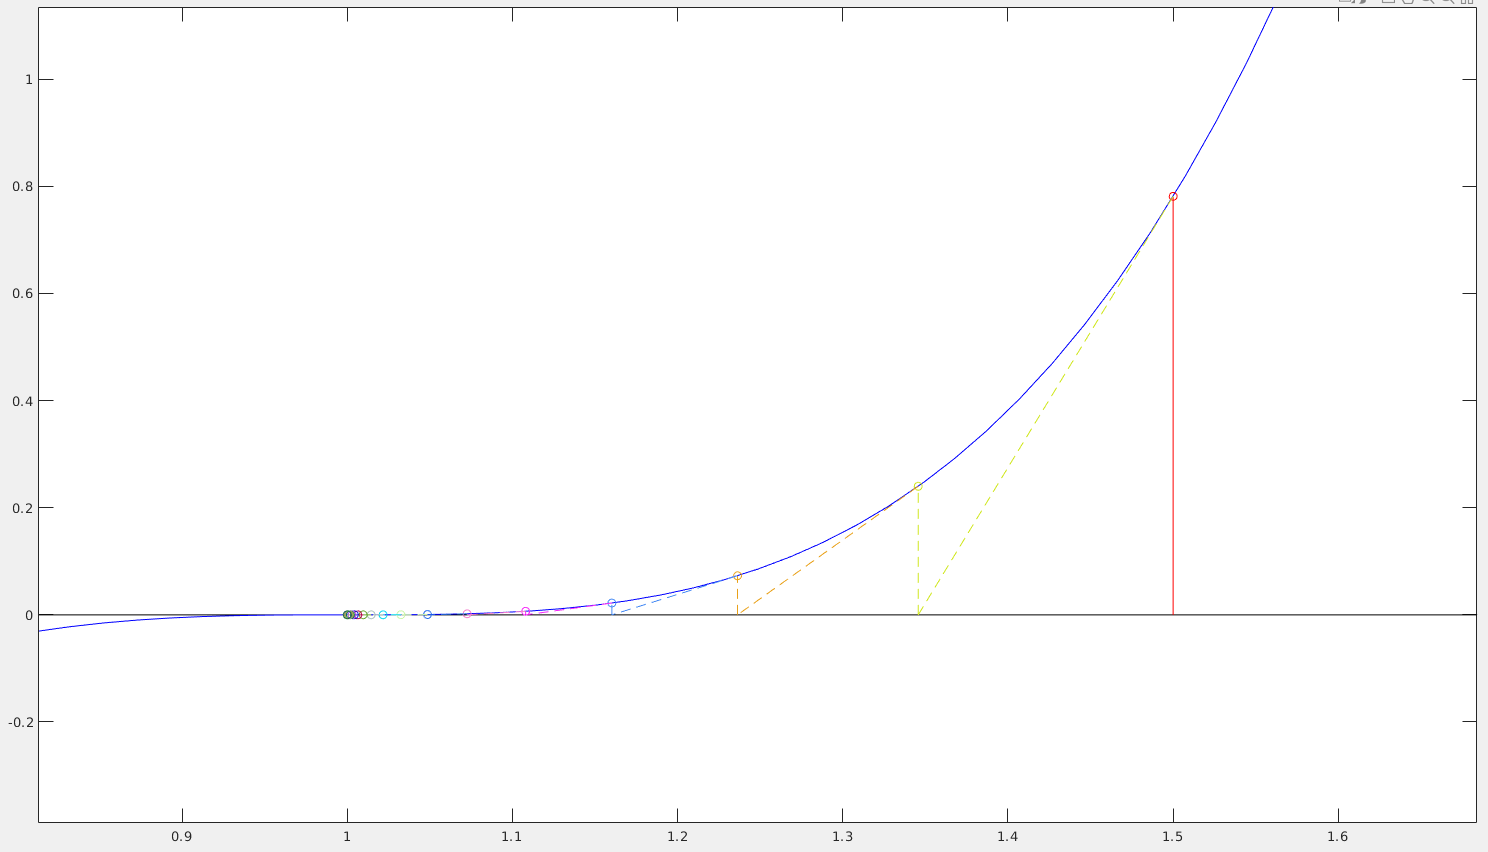
\includegraphics[scale=0.40]{MultiRadixNewton.png}
    \caption{Grafico Metodo delle corde su $f(x)=x^5-3x^4+7x^3-13x^2+12x-4$}
\end{figure} \\
Questi sono i risultati ottenuti dall'esecuzione del programma in MATLAB.\\ Come si può vedere,l'algoritmo esegue più di 100 iterazioni andando a passare come parametro una tolleranza pari a $10^{-8}$.
Il risultato \'e dovuto al fatto che non va ad aggiornare $f'(x)$ ogni volta, ma lo calcola solo inizialmente. Quindi avendo la sempre la solita derivata, ci mette più iterazioni rispetto al metodo di Newton.

\newpage

\subsubsection{Metodo delle Secanti}
Con il metodo delle Secanti, andando a dare come parametri $f(x)=x^5-3x^4+7x^3-13x^2+12x-4$, $x_0=  1.5$ e $x_1=1.6$ otteniamo:
\begin{figure}[ht!]
    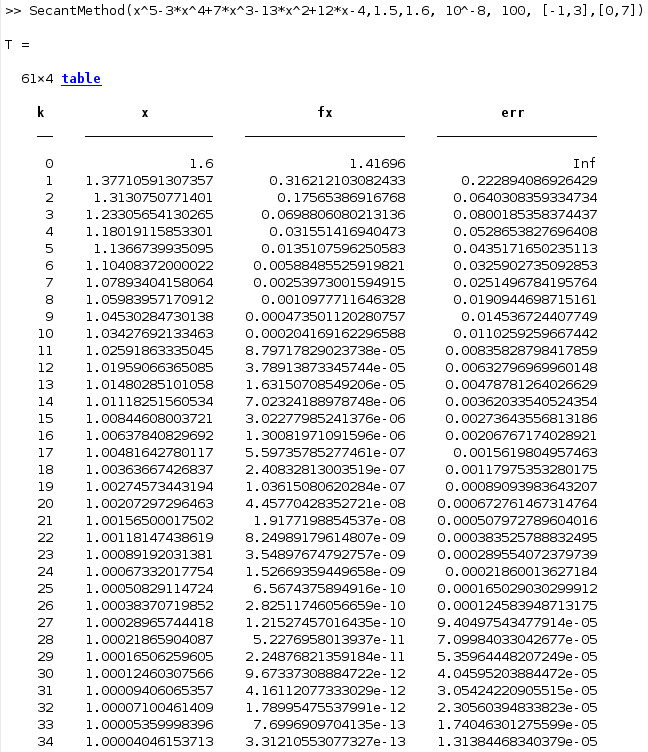
\includegraphics[scale=0.7]{TabellaMultiRadixSecant1.png}
    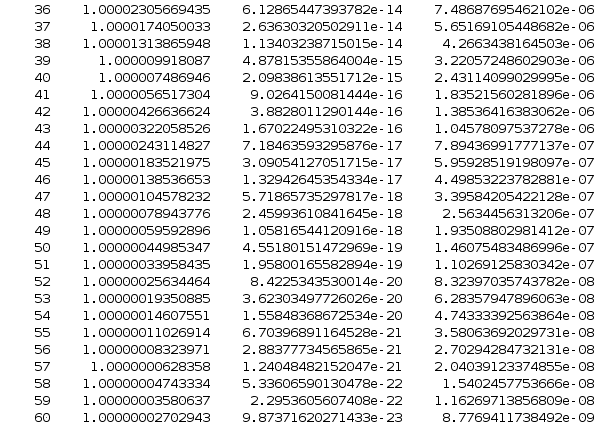
\includegraphics[scale=0.7  ]{TabellaMultiRadixSecant2.png}
    \caption{Tabella Metodo delle Secanti, su $f(x)=x^5-3x^4+7x^3-13x^2+12x-4$}
\end{figure}
\begin{figure}[ht!]
    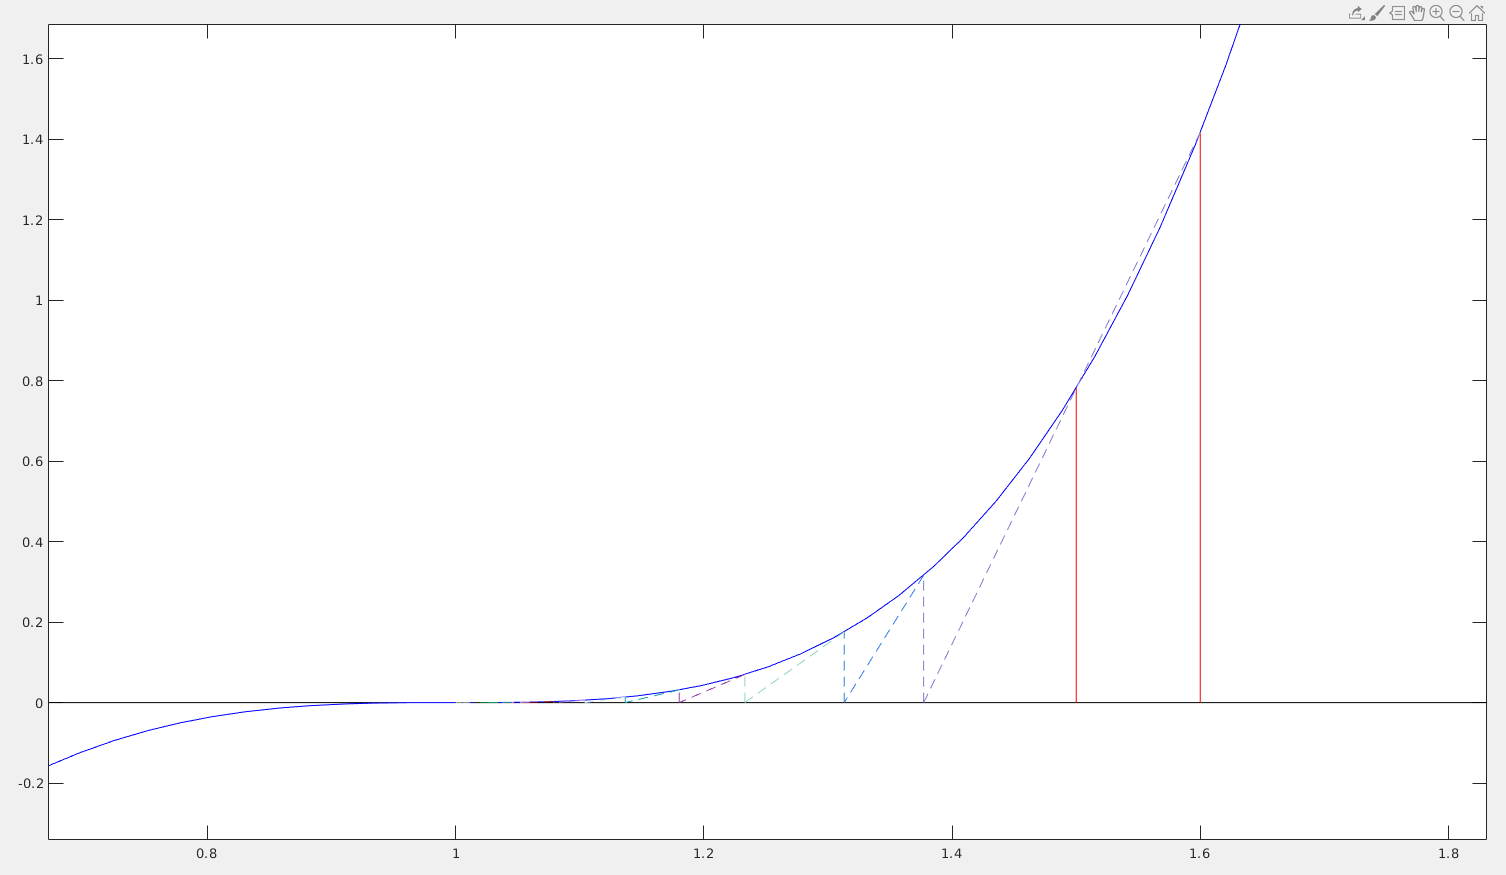
\includegraphics[scale=0.43]{MultiRadixSecantMethod.png}
    \caption{Grafico Metodo delle corde su $f(x)=x^5-3x^4+7x^3-13x^2+12x-4$}
\end{figure}
Questi sono i risultati ottenuti dall'esecuzione del programma in MATLAB.\\ Come si può vedere,l'algoritmo esegue 60 iterazioni andando a passare come parametro una tolleranza pari a $10^{-8}$.
Usando due punti iniziali, riesce ad approssimare, come si \'e visto prima, con velocit\'a di convergenza superlineare, quindi più veloce rispetto al metodo delle corde.


\subsection{Conclusioni}
Come ci aspettavamo dalla descrizione data dei vari metodi per la ricerca degli zeri, il metodo di Newton \'e il più veloce tranne nel caso delle radici multiple.
Il metodo di punto fisso, può convergere sia linearmente che quadraticamente. Nel caso $e^{-x}-2x^2$ convergeva linearmente, infatti \'e stato più lento rispetto ai $2$ metodi Quasi-Newton.
Infine il metodo di Bisezione \'e il metodo più lento tra tutti quelli descritti, questo perch\'e compie un numero di iterazioni gi\'a conosciuto pari a: $k \geq \lceil log_2(\frac{b-a}{\epsilon}) \rceil$. Questo numero può essere significativamente elevato richidendo 
molte valutazioni della funzione $f$.

\newpage

\section{Codice MATLAB}
\subsection{Metodo di Bisezione}
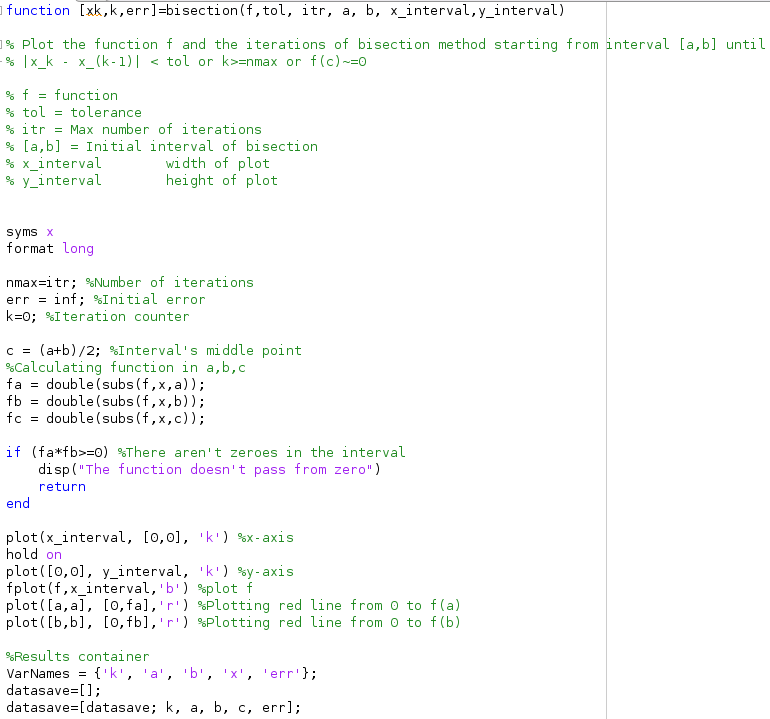
\includegraphics[scale=0.78]{ProgrammaBisezione1.png}\\
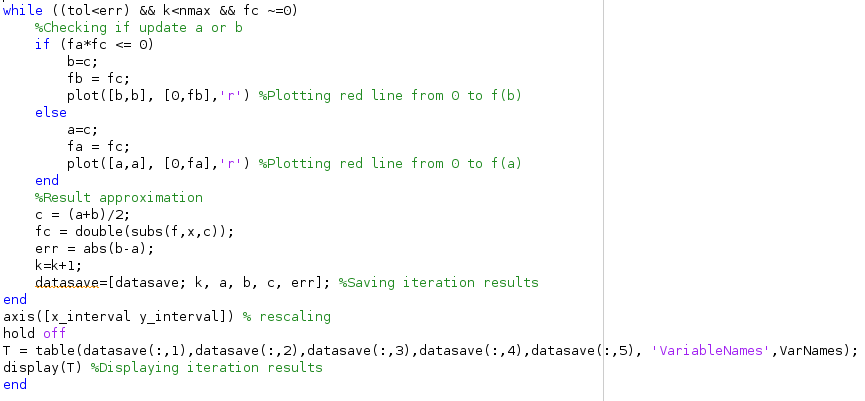
\includegraphics[scale=0.78]{ProgrammaBisezione2.png}

\subsection{Metodo di Punto Fisso}
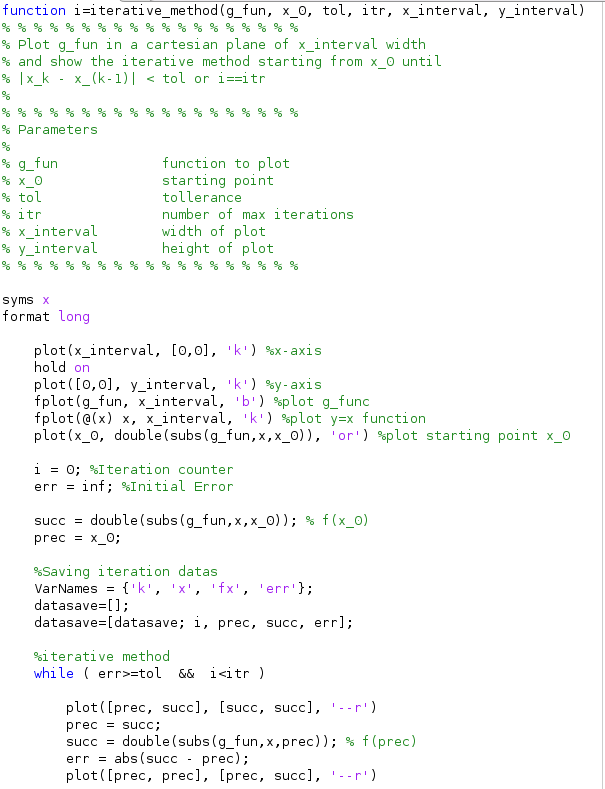
\includegraphics[scale=0.83]{ProgrammaPuntoFisso1.png}\\
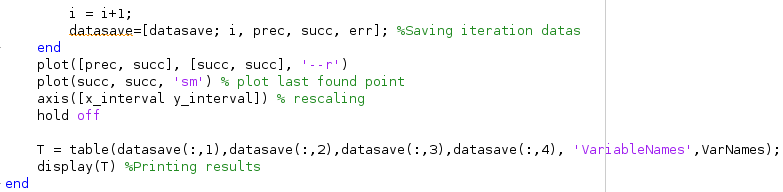
\includegraphics[scale=0.83]{ProgrammaPuntoFisso2.png}
\newpage

\subsection{Metodo di Newton}
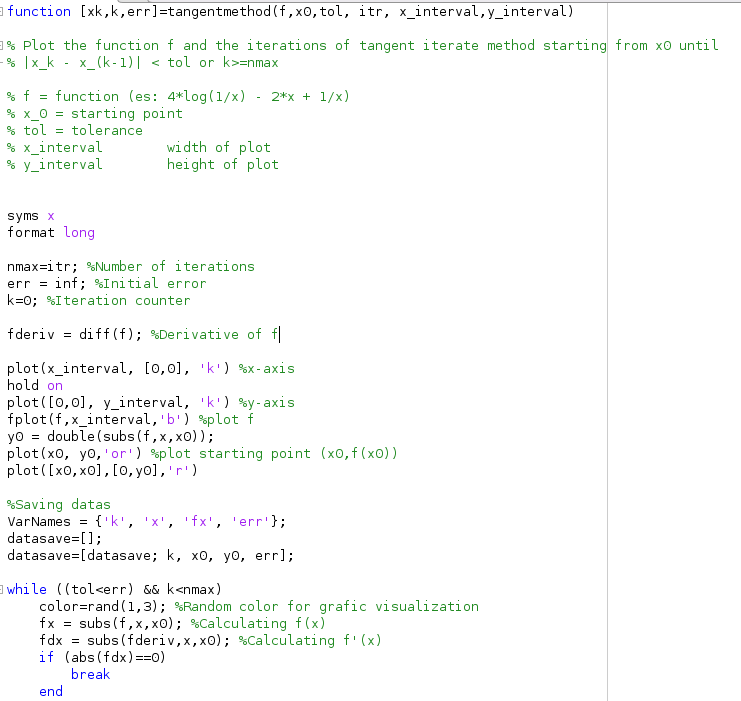
\includegraphics[scale=0.86]{ProgrammaNewton1.png}\\
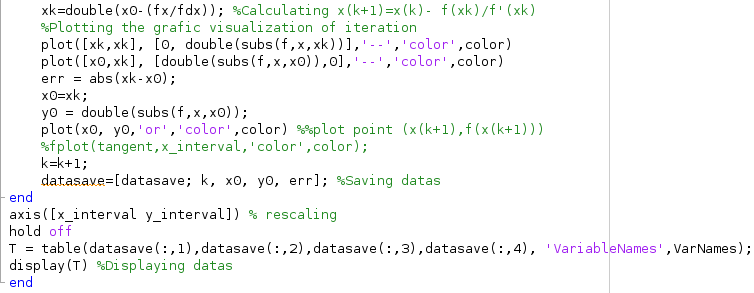
\includegraphics[scale=0.86]{ProgrammaNewton2.png}
\newpage

\subsection{Metodo delle Corde}
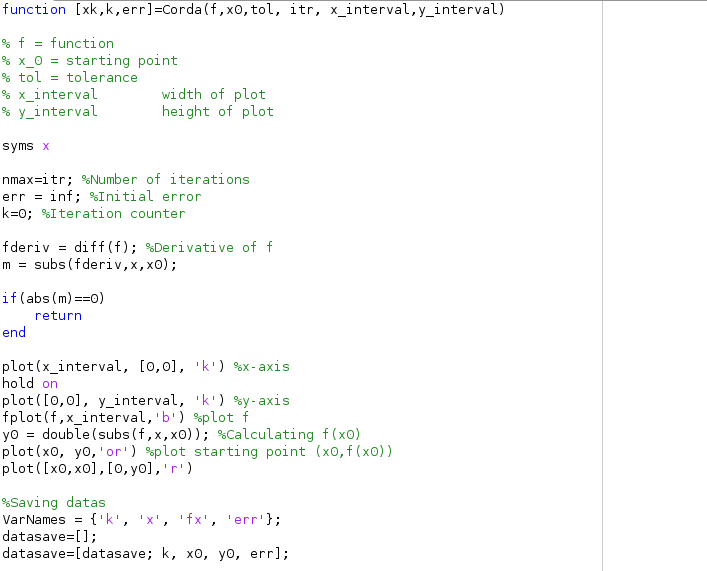
\includegraphics[scale=0.86]{ProgrammaCorda1.png}\\
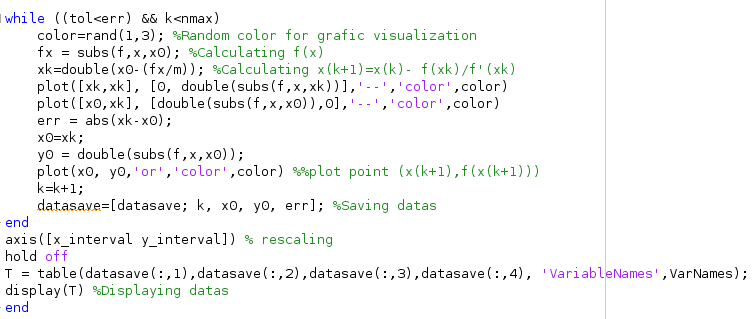
\includegraphics[scale=0.86]{ProgrammaCorda2.png}
\newpage

\subsection{Metodo delle Secanti}
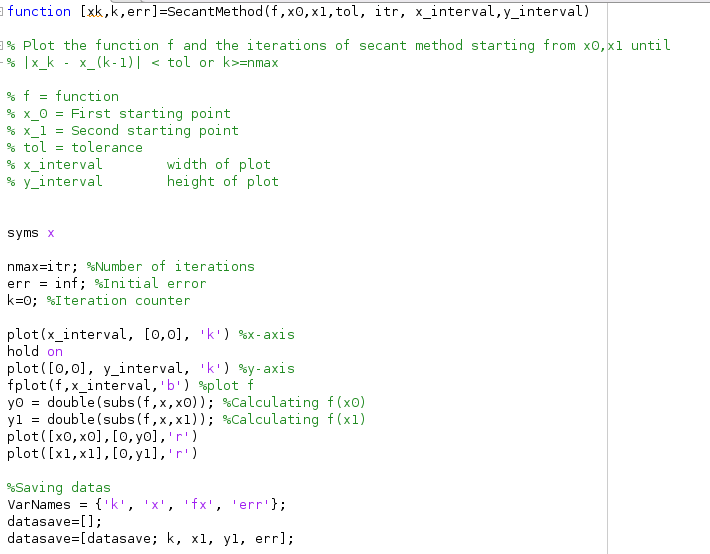
\includegraphics[scale=0.86]{ProgrammaSecanti1.png}\\
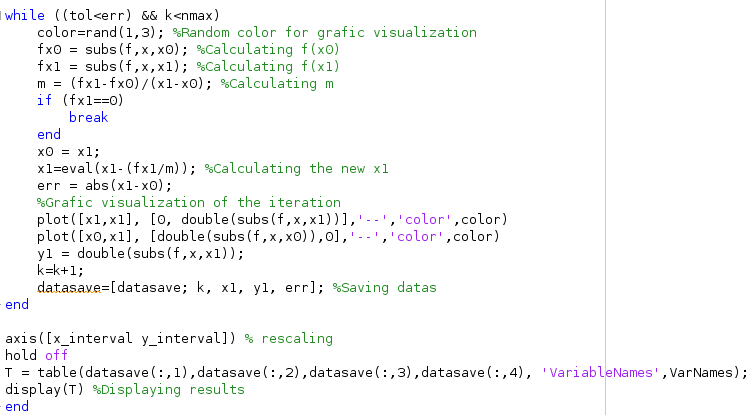
\includegraphics[scale=0.86]{ProgrammaSecanti2.png}
\newpage

\newpage
\nocite{*}
\printbibliography[heading=bibintoc,type=book,title={Bibliografia}] 
\printbibliography[heading=bibintoc,type=online,title={Sitografia}]





\end{document}
